% The dvipsnames option is passed to the xcolor package, which beamer loads
\documentclass[xcolor={dvipsnames}]{beamer}

\usepackage{smpa2152-style}

\title[Political Polling]{Political Polling -- Part I: \\ Evolution of Polling}
\author[SMPA 2152]{Data Analysis for Journalism and Political Communication (Fall 2025)}
\date{Prof. Bell}

\begin{document}

%%%%%%%%%%%%%%%%%%%%%%%%%%%%%%%%%%%%%%%%%%%%%%%%%%%%%%%%%%%%%%%%%%
\titlegraphic{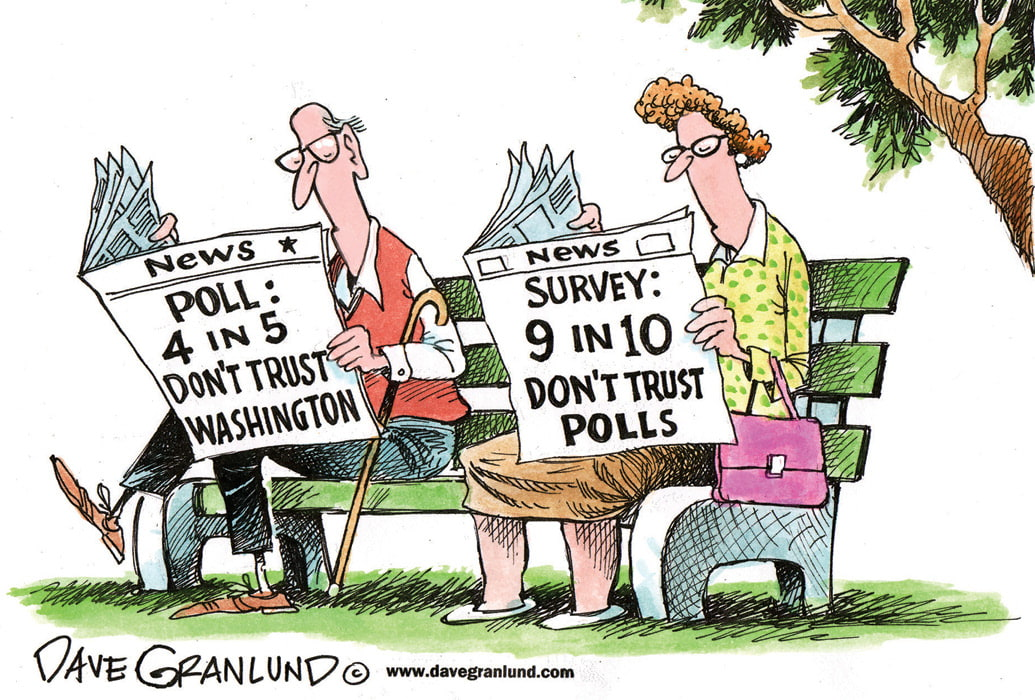
\includegraphics[width=.4\textwidth]{pollsters_political_cartoon.jpg}}
\frame{
\titlepage
}

%%%%%%%%%%%%%%%%%%%%%%%%%%%%%%%%%%%%%%%%%%%%%%%%%%%%%%%%%%%%%%%%%%
\frame{\frametitle{When Polling Misses}

\only<1>{
\centering
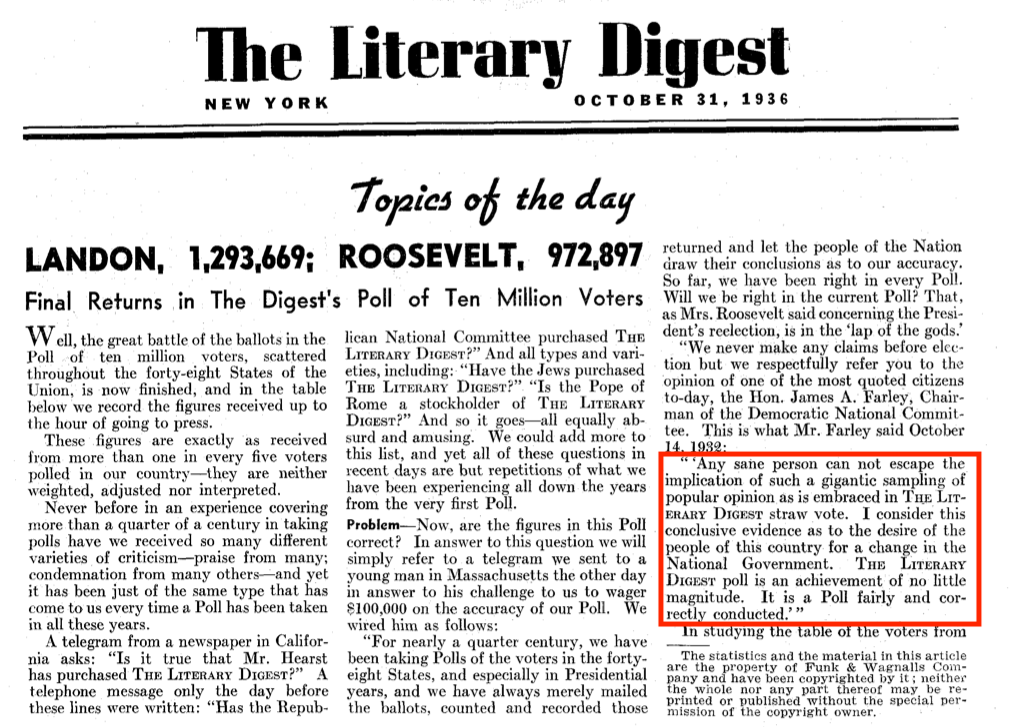
\includegraphics[width=.9\textwidth]{literary_digest_landon_roosevelt.png}}

\only<2>{
\begin{columns}[c, onlytextwidth]
    \begin{column}{.6\textwidth}
        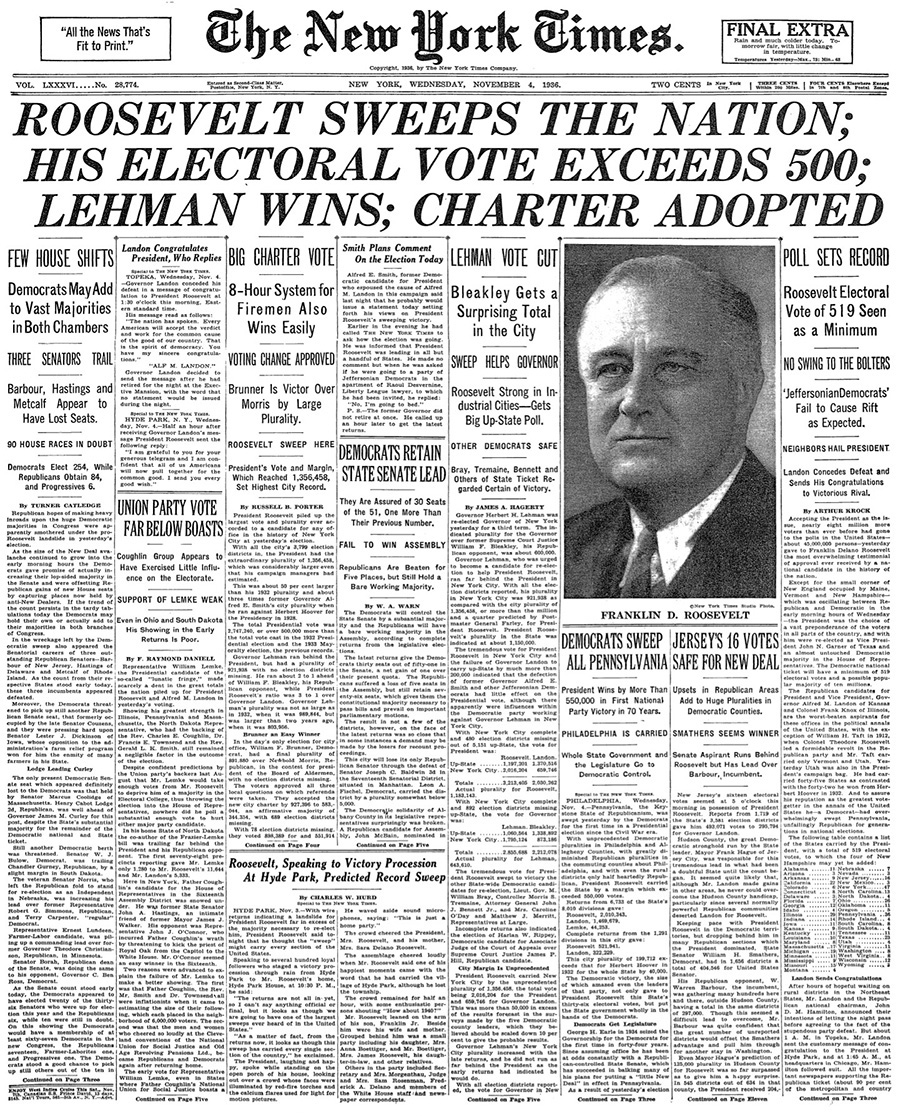
\includegraphics[height=.9\textheight]{1936nyt.jpg}
    \end{column}
    \begin{column}{.4\textwidth}
    \begin{center}
        
\includegraphics[width=.9\textwidth]{literary_digest_face_red.jpg}
    \end{center}
    \end{column}
\end{columns}}

\only<3>{
\centering
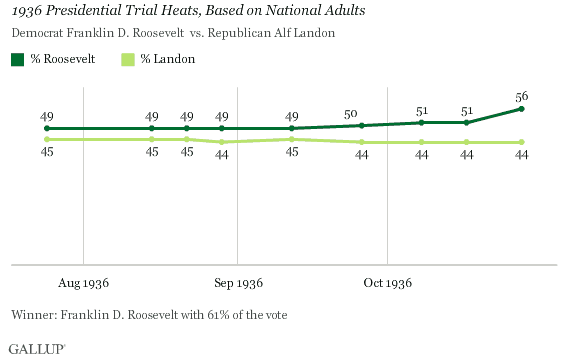
\includegraphics[width=.9\textwidth]{1936_gallup_polls.png}}

\only<4>{
\centering
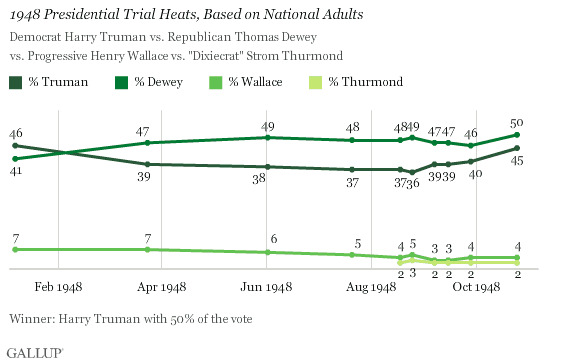
\includegraphics[width = .9\textwidth]{1948GallupPolls.jpg}}

\only<5>{
\centering
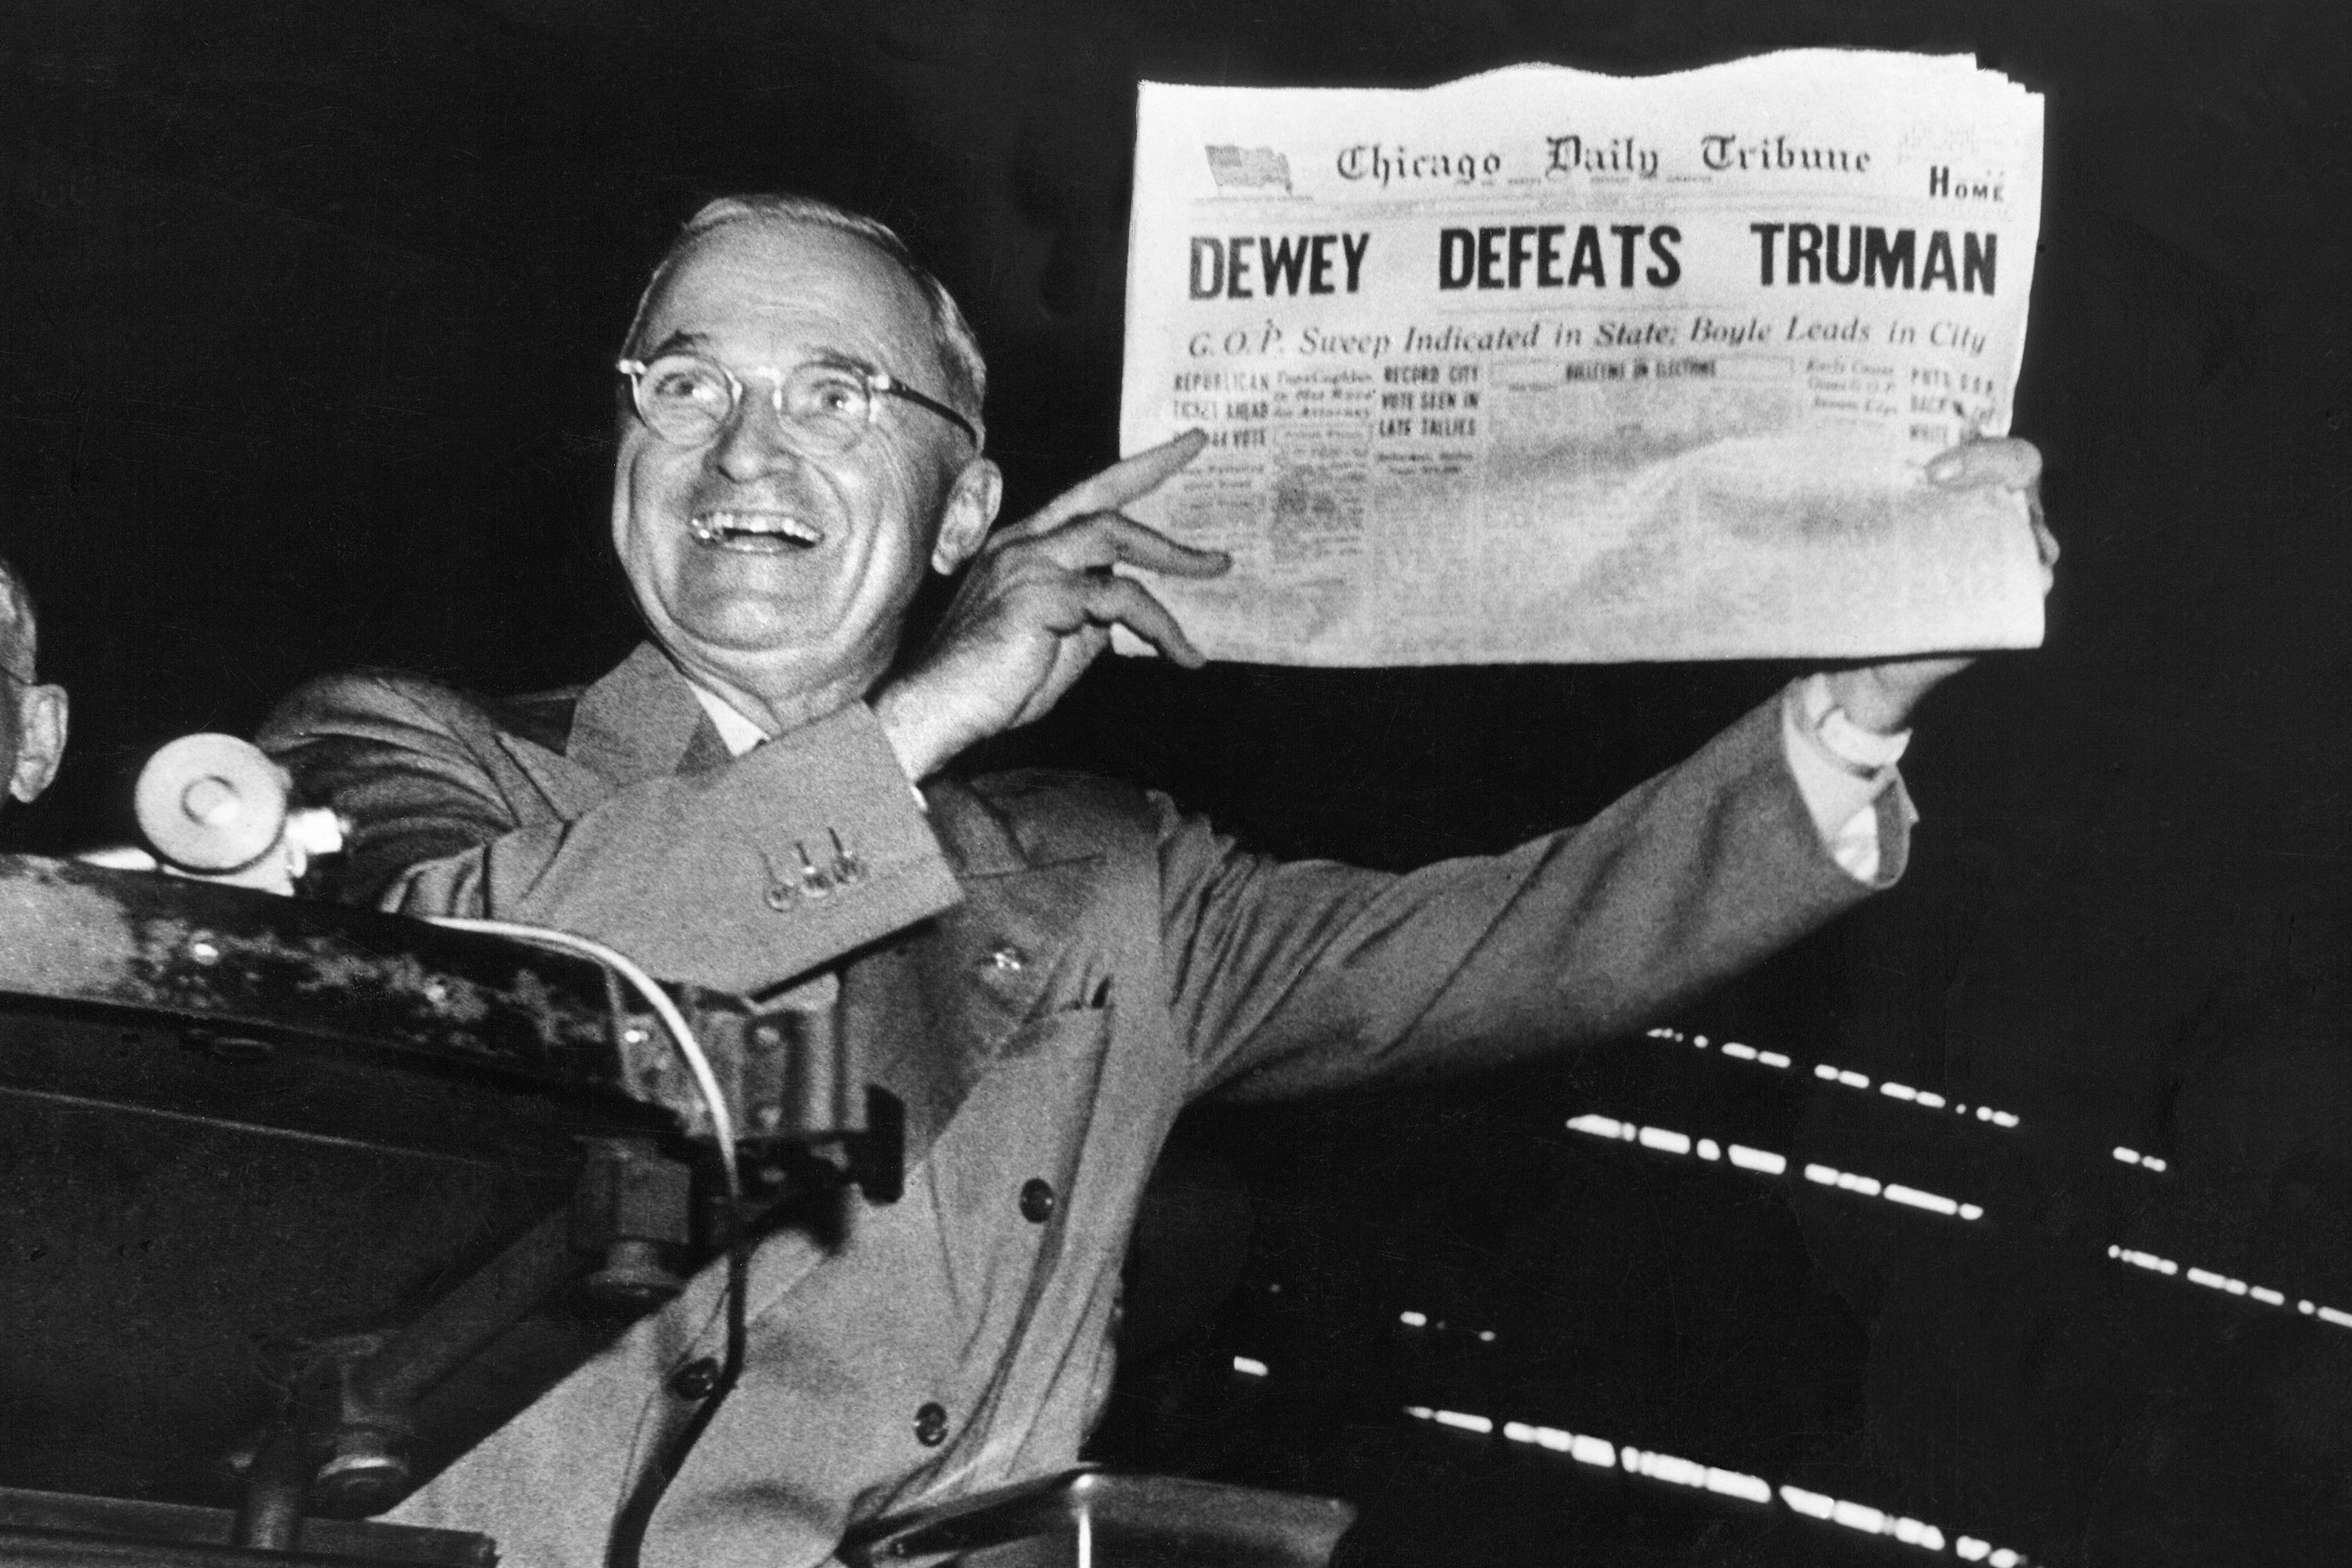
\includegraphics[width = .9\textwidth]{dewey_defeats_truman.jpg}}
}

%%%%%%%%%%%%%%%%%%%%%%%%%%%%%%%%%%%%%%%%%%%%%%%%%%%%%%%%%%%%%%%%%%
\frame{\frametitle{The 2016 Election Polls}

\only<1>{
\centering
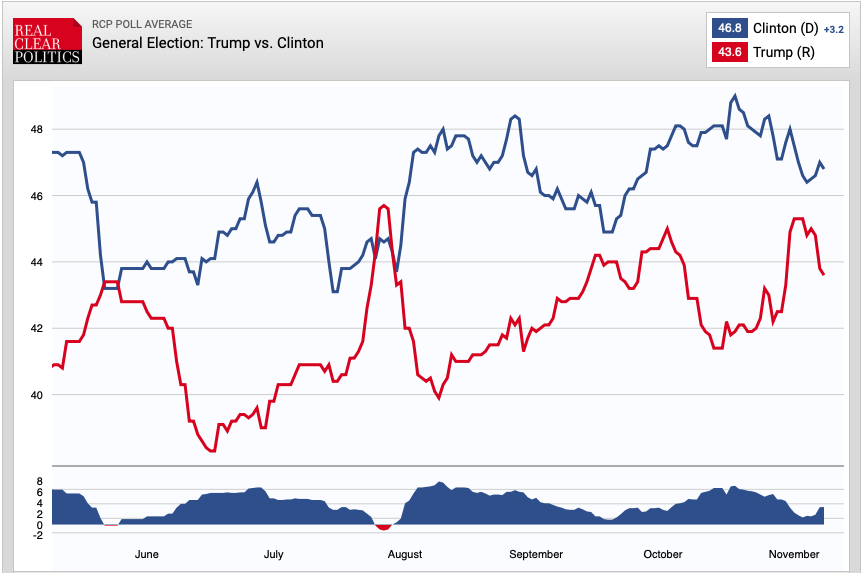
\includegraphics[width = .9\textwidth]{RCP2016Election.png}}

\only<2,4>{
\begin{enumerate}[<+(1)->]
    \item The polls weren't that wrong
    \item<4> The polls were wrong due to non-response bias, a form of selection bias
\end{enumerate}}

\only<3>{
    \centering
    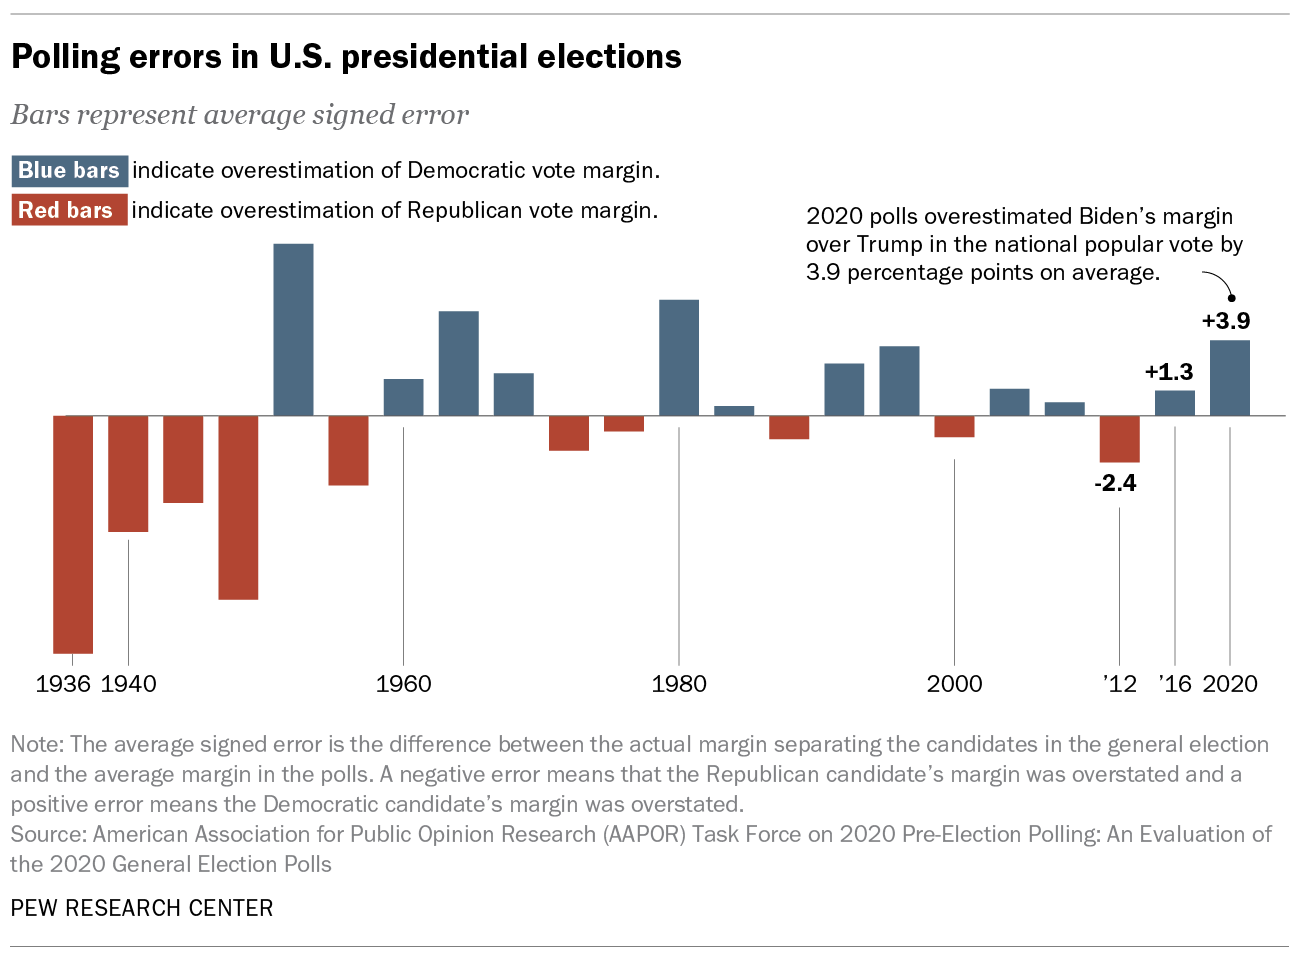
\includegraphics[width = .8\textwidth]{historical_polling_error.png}}

\only<4>{
    \centering
    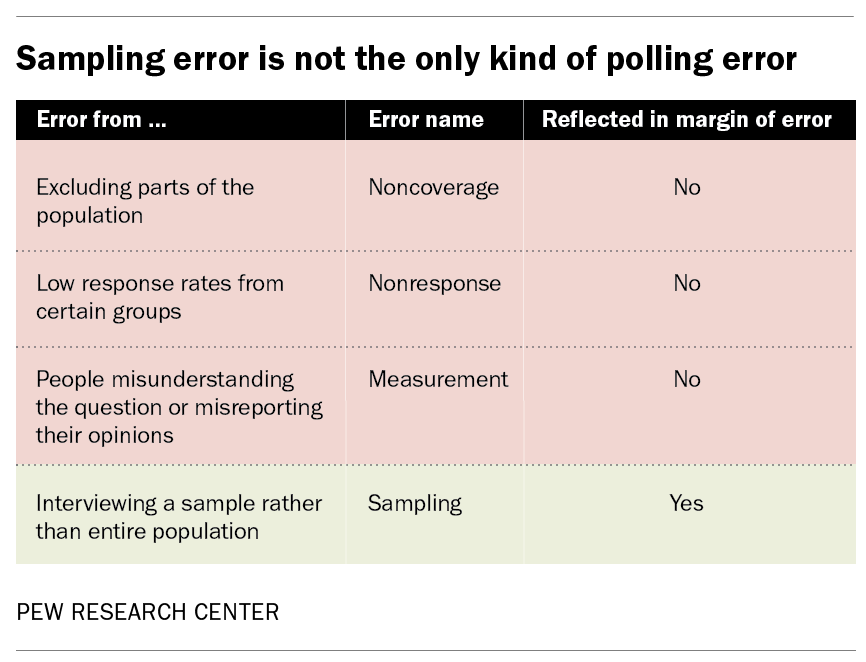
\includegraphics[width = .6\textwidth]{polling_errors.png}}
}

%%%%%%%%%%%%%%%%%%%%%%%%%%%%%%%%%%%%%%%%%%%%%%%%%%%%%%%%%%%%%%%%%%
\frame{\frametitle{Types of Missing Data}

\only<1-4,6->{
\begin{itemize}[<+->]
    \item \textbf{Missing Completely at Random (MCAR)}: Observations are missing for non-systematic reasons
    \item \textbf{Missing at Random (MAR)}: Missing observations are correlated with a factor other than the outcome that is being measured
    \begin{itemize}
        \item MAR data can be resolved using a statistical technique called ``weighting'' in which answers from less-responsive groups are counted more, and answers from more-responsive groups are counted less
        \item Like making a ``public opinion soup'' but can go wrong (e.g., LA Times)
    \end{itemize}
    \item<6-> \textbf{Missing Not at Random (MNAR)}: Missing outcomes are correlated with the outcome that is being measured
    \begin{itemize}
        \item<7-> MNAR data is a challenge because the only thing that predicts what data is missing is the fact that it is missing
    \end{itemize}
\end{itemize}
}

\only<5>{
\centering
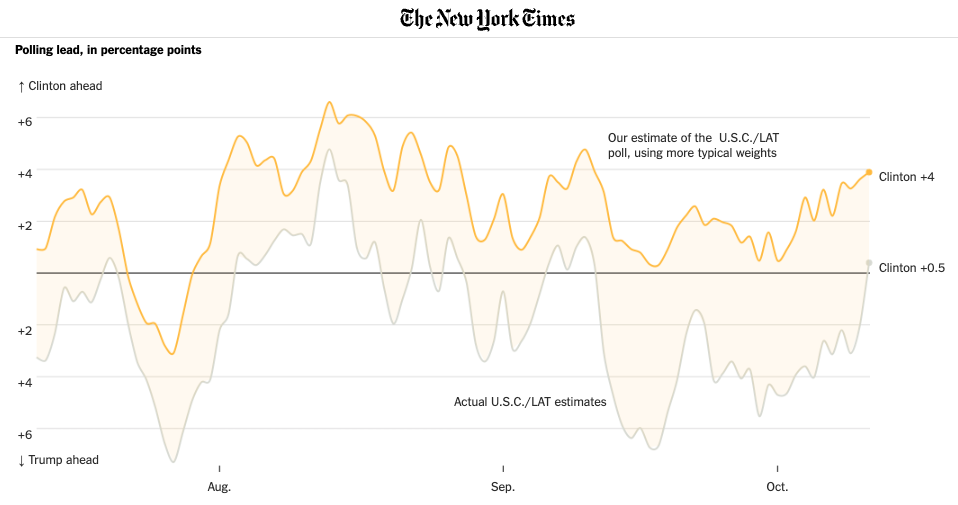
\includegraphics[width = .9\textwidth]{latimes.png}}
}

%%%%%%%%%%%%%%%%%%%%%%%%%%%%%%%%%%%%%%%%%%%%%%%%%%%%%%%%%%%%%%%%%%
\frame{\frametitle{The 2016 Election Polls}

\only<1>{
\begin{enumerate}
    \item The polls weren't that wrong
    \item The polls were wrong due to \textbf{missing at random (MAR)} non-response bias by education
\end{enumerate}}

\only<2>{
\centering
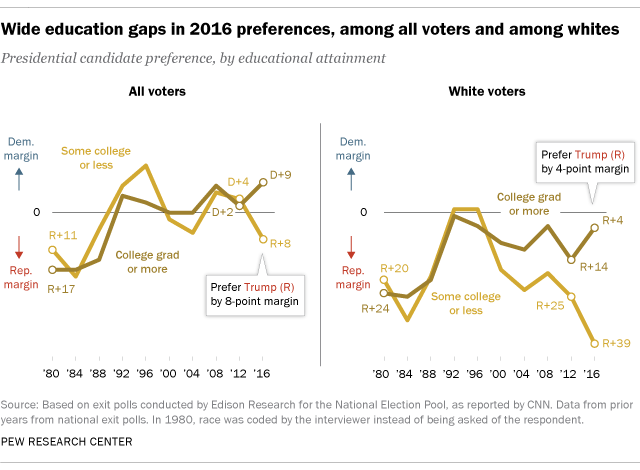
\includegraphics[width = .9\textwidth]{2016_education_votechoice.png}}

\only<3>{
\centering
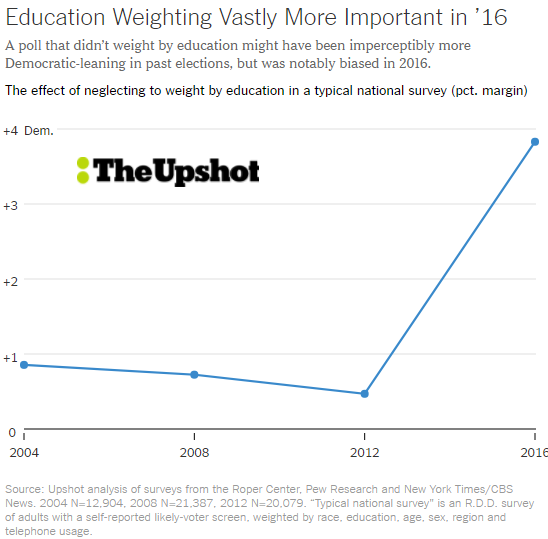
\includegraphics[width = .65\textwidth]{2016_education_weighting.png}}

}

%%%%%%%%%%%%%%%%%%%%%%%%%%%%%%%%%%%%%%%%%%%%%%%%%%%%%%%%%%%%%%%%%%
\frame{\frametitle{The 2020 Election Polls}

\only<1>{
\centering
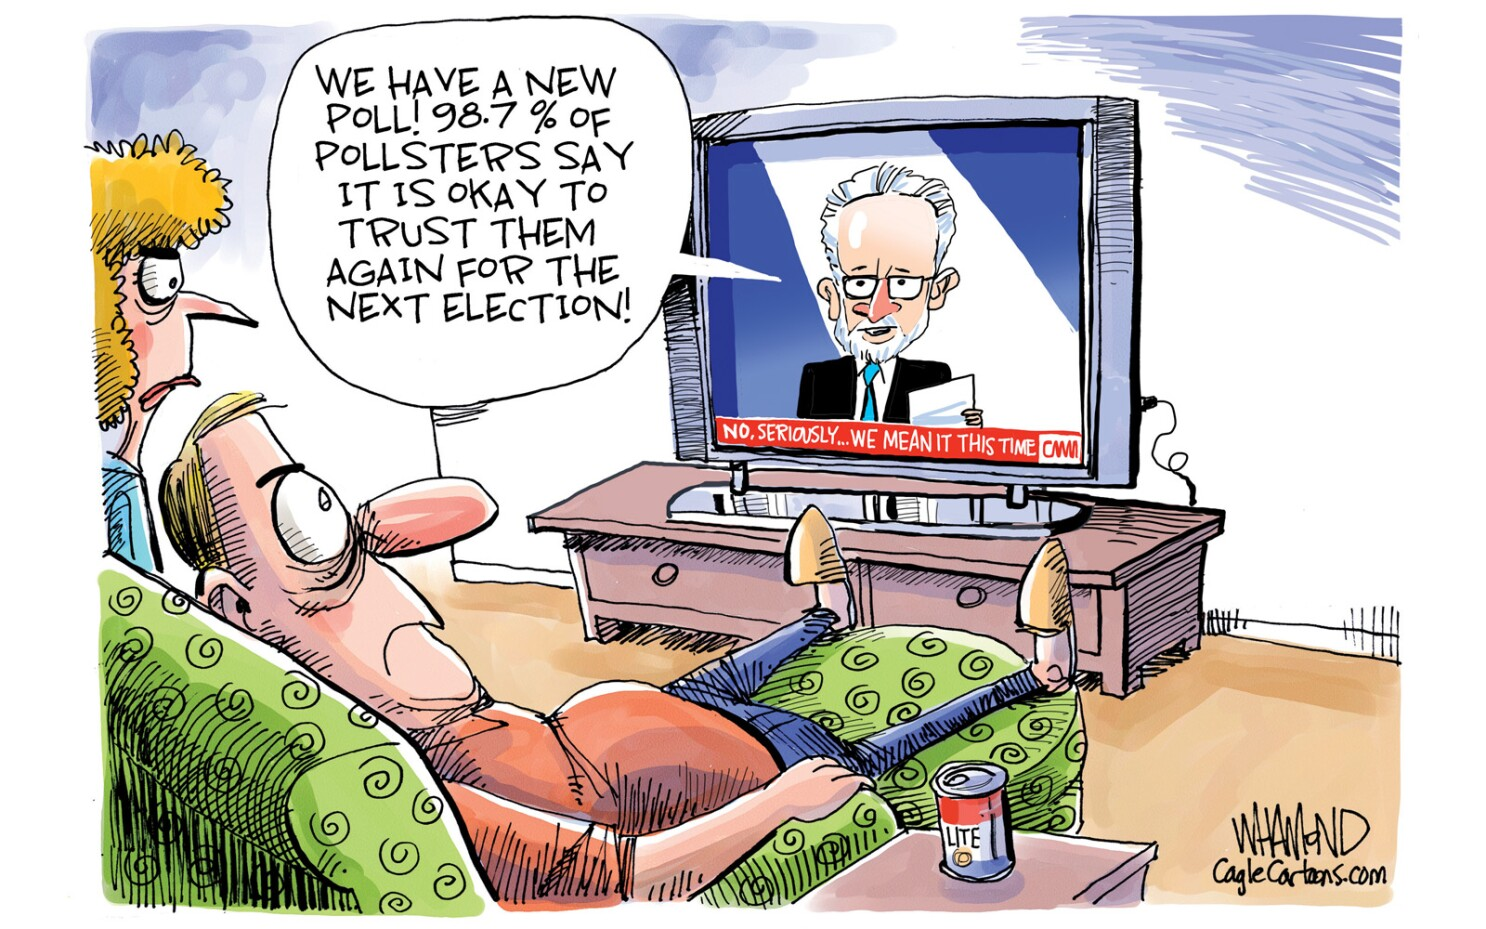
\includegraphics[width = .9\textwidth]{pollsters_trust_us_again.jpg}}

\only<2>{
\centering
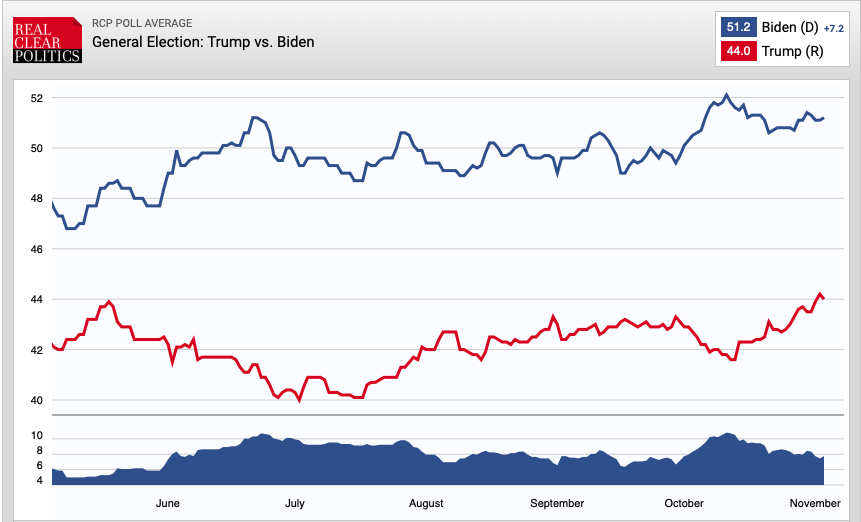
\includegraphics[width = .9\textwidth]{RCP2020Election.png}}

\only<3-5,7-8,10>{
    \begin{enumerate}[<+(2)->]
        \item The polls weren't that wrong (again)
        \item It is challenging to poll during a pandemic and with record-high turnout (the models were wrong)
        \item The polls were wrong due to missing at random (MAR) non-response bias (again)
        \item<7-> The polls were wrong due to \textbf{missing not at random (MNAR)} non-response bias
        \begin{itemize}[<+->]
            \item<8-> ``Shy Trump voters'' theory
            \item<10> Trump voters are less likely to respond to surveys
        \end{itemize}
    \end{enumerate}
}

\only<6>{
\centering
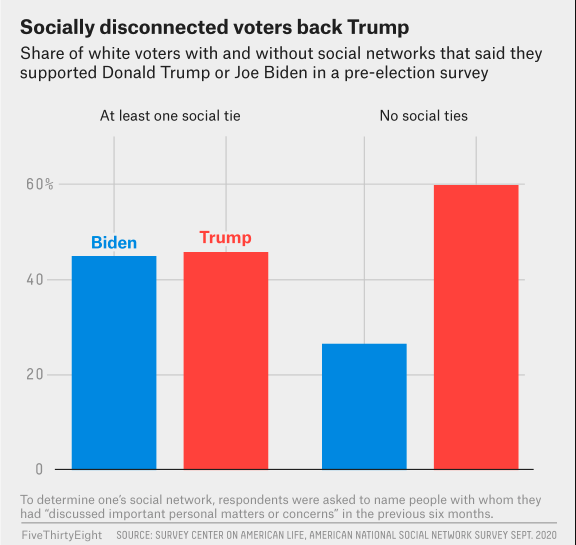
\includegraphics[height = .8\textheight]{social_ties.png}}

\only<9>{
\centering
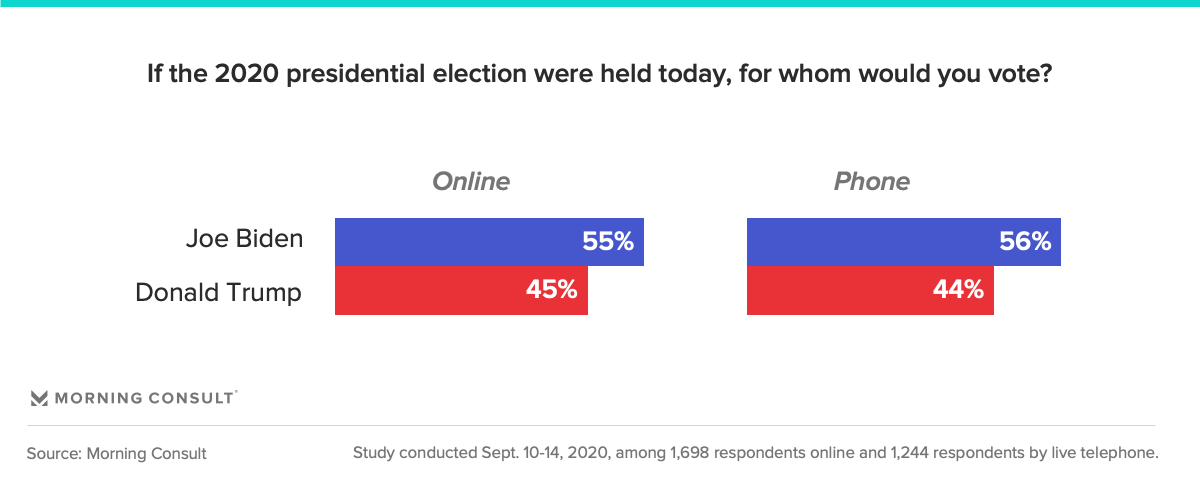
\includegraphics[width = .9\textwidth]{shy_trump.png}}

\only<11>{
\centering
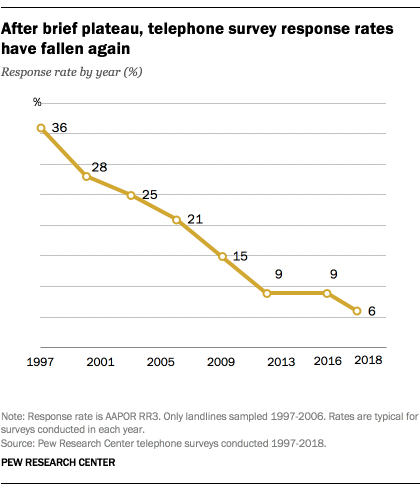
\includegraphics[width = .5\textwidth]{phone_response_rate.png}}

\only<12>{
\centering
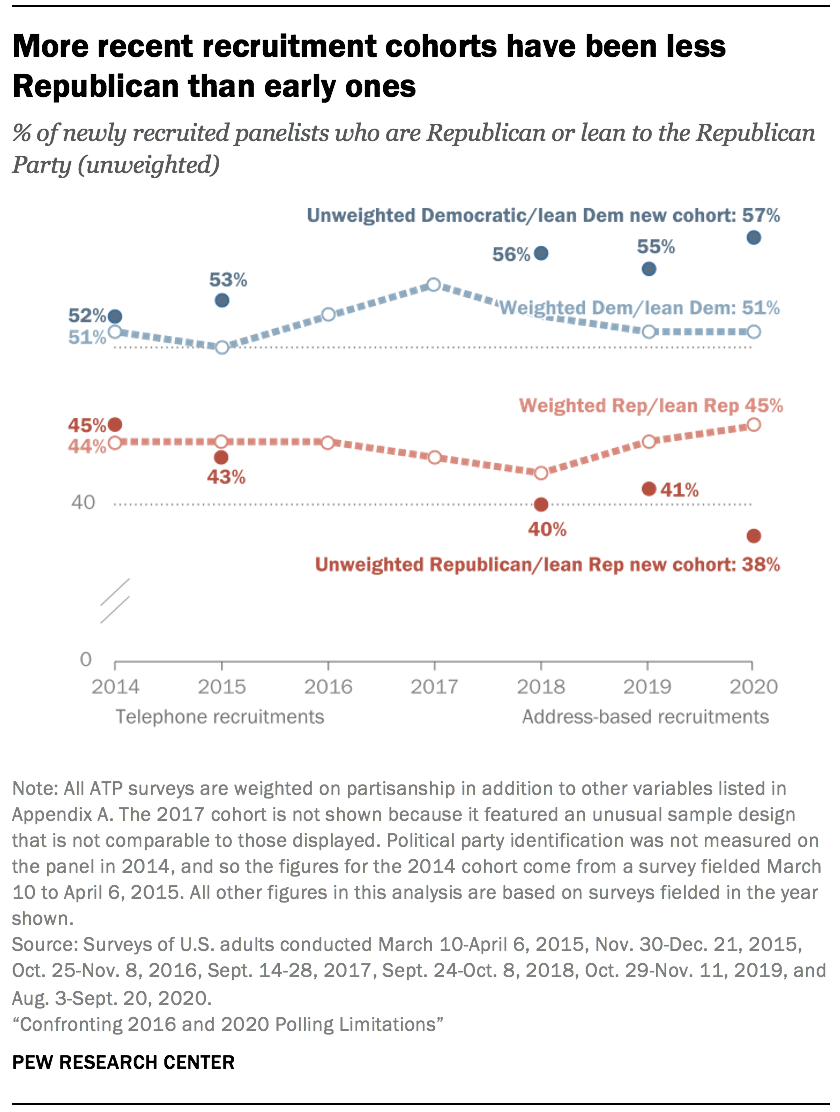
\includegraphics[width = .5\textwidth]{ATP_fewer_republicans.png}}
}

%%%%%%%%%%%%%%%%%%%%%%%%%%%%%%%%%%%%%%%%%%%%%%%%%%%%%%%%%%%%%%%%%%
\frame{\frametitle{The 2022 Election Polls}

\only<2>{
    \centering
    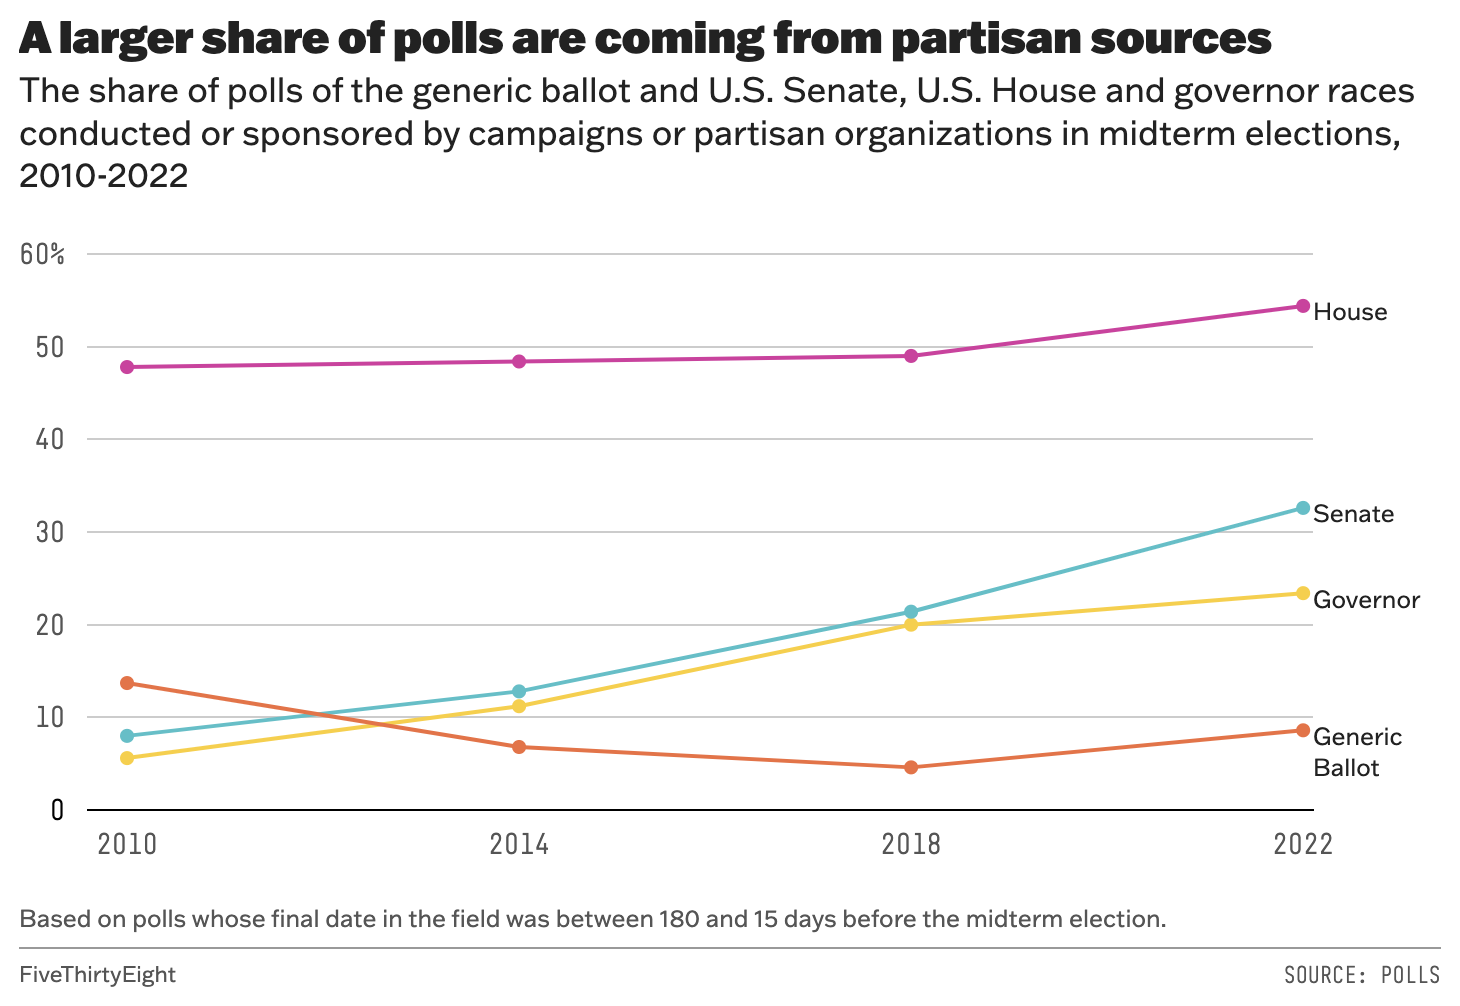
\includegraphics[width = .9\textwidth]{partisan_polls.png}
}

\only<3>{
    \centering
    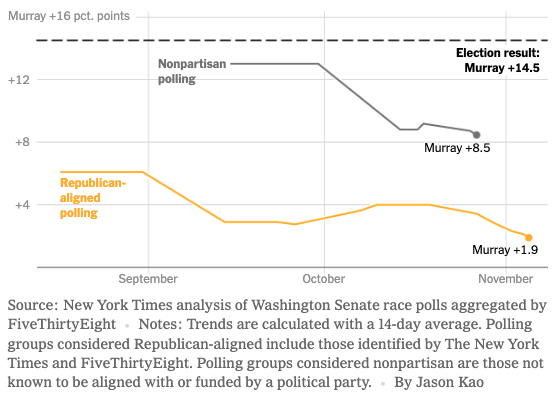
\includegraphics[width = .9\textwidth]{patty_murray.png}
}

\only<5>{
    \centering
    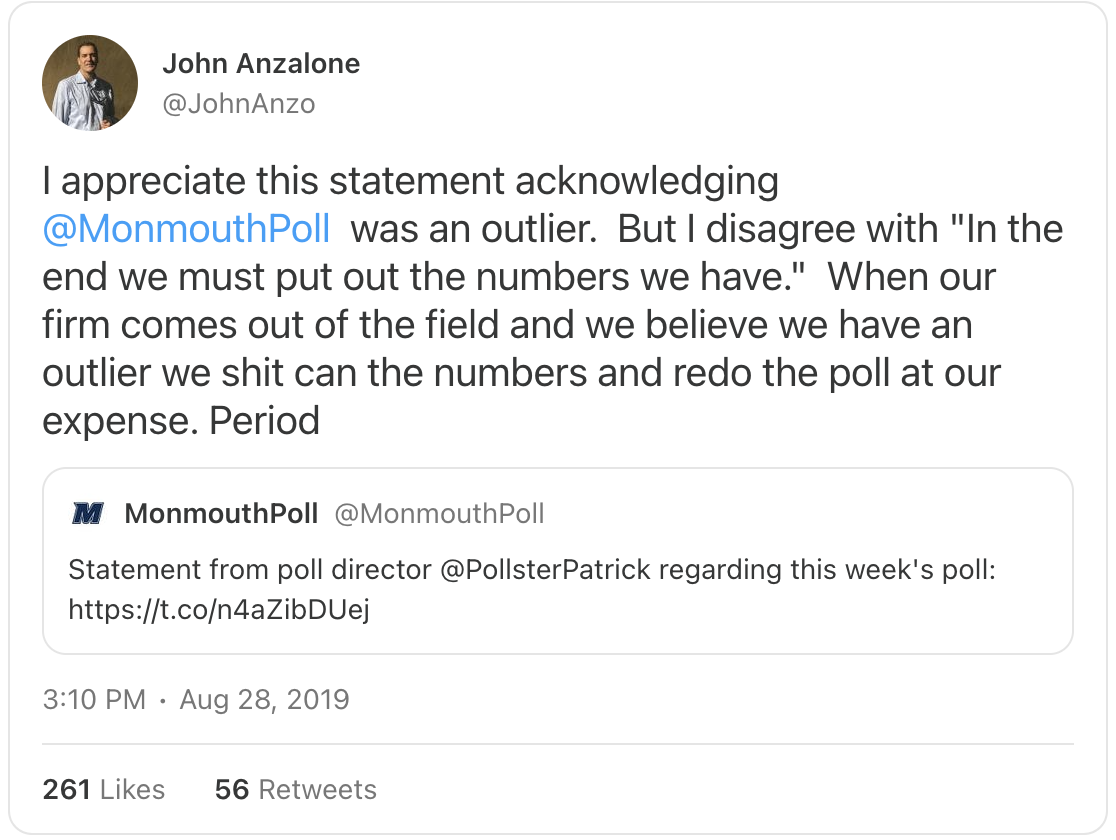
\includegraphics[height = .8\textheight]{herding.png}
}

\only<8>{
    \centering
    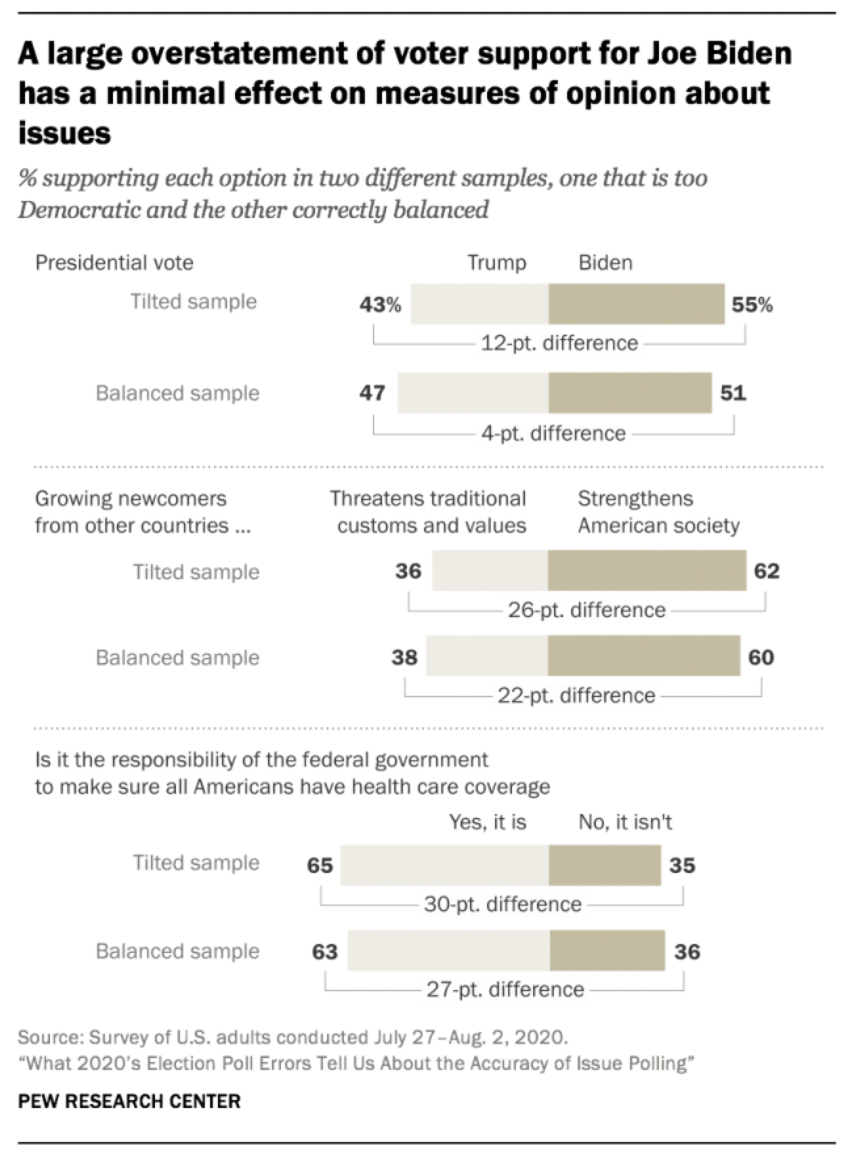
\includegraphics[height = .8\textheight]{issue_polling.png}
}

\only<1,4,6-7>{
    \begin{enumerate}[<+->]
        \item Republican-aligned pollsters were over-represented in polling averages, creating an expectation of a ``red wave''
        \item<4-> Pollsters engaged in \textbf{herding} -- adjusting the results of their findings to more closely match the results of other polls (or not releasing outlying polls at all) -- to avoid being wrong
        \item<6-> Something is unique about elections in which Donald Trump is a candidate
        \begin{itemize}
            \item<7-> Issue polling seems to be unaffected by biases influencing horse race polling
        \end{itemize}
    \end{enumerate}
}
}

%%%%%%%%%%%%%%%%%%%%%%%%%%%%%%%%%%%%%%%%%%%%%%%%%%%%%%%%%%%%%%%%%%
\frame{\frametitle{The 2024 Election Polls}

\only<1>{
    \centering
    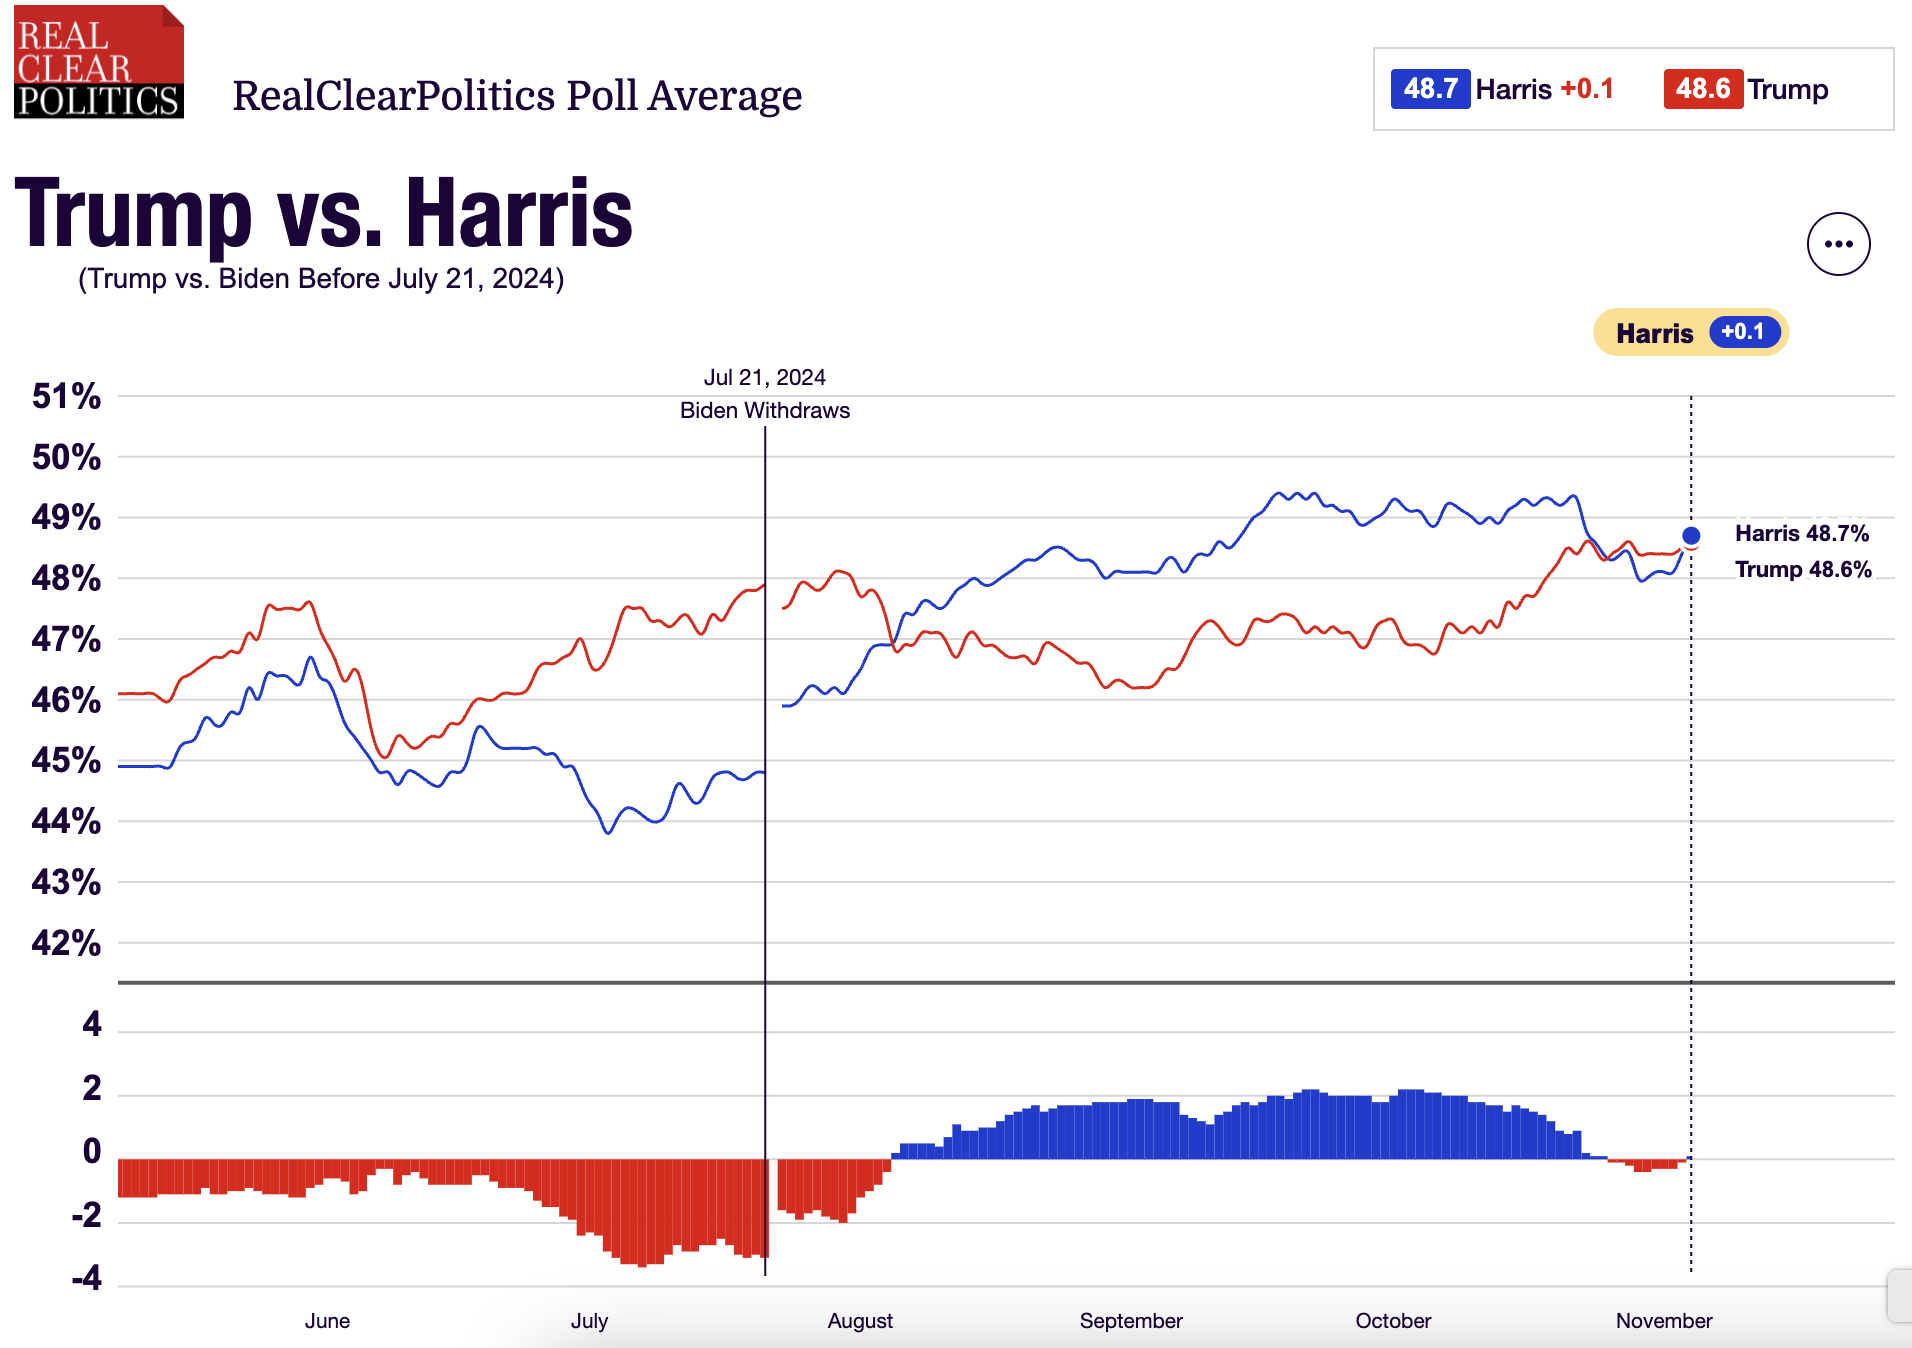
\includegraphics[width = .8\textwidth]{RCP2024Election.png}
}

\only<2>{
    \centering
    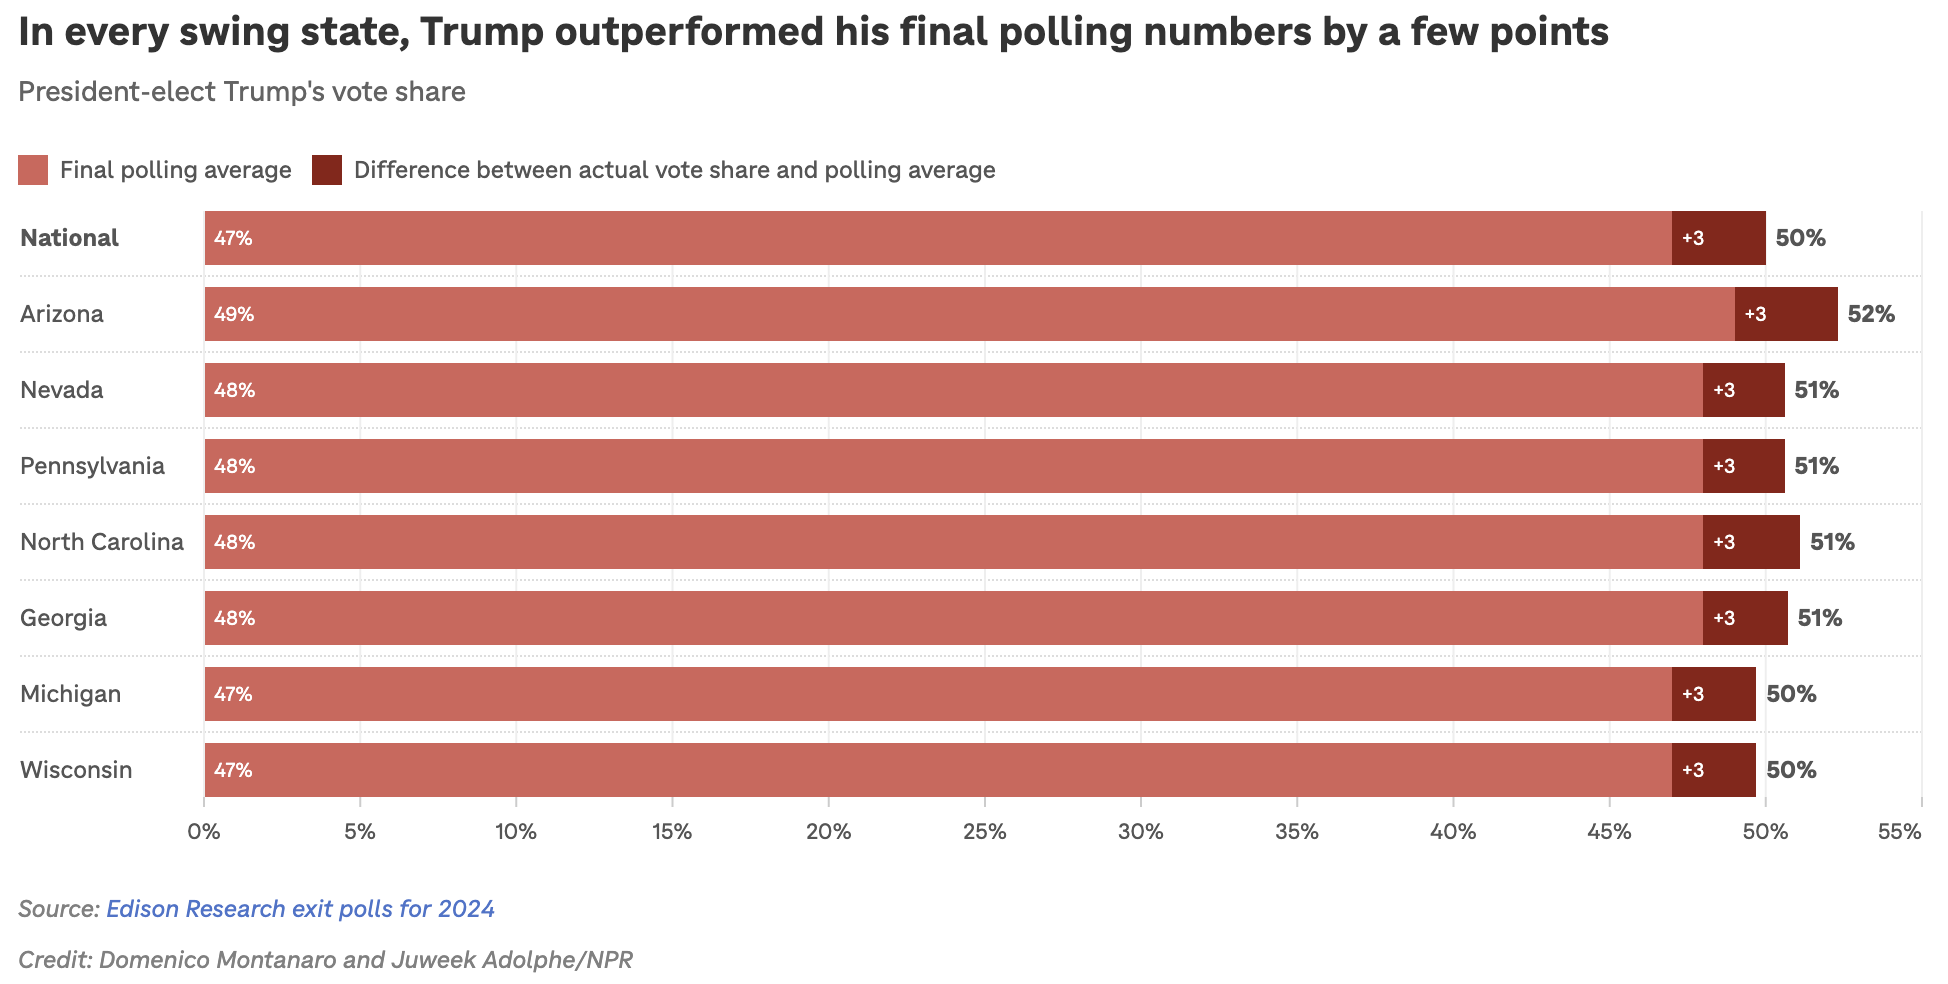
\includegraphics[width = .9\textwidth]{2024_swing_state_errors.png}
}

\only<3-4>{
    \begin{itemize}
        \item Pollsters used new techniques to address partisan non-response, like weighting on \textbf{recalled vote}
    \end{itemize}
}

\only<3> {
    \centering
    ~\\
    \fbox{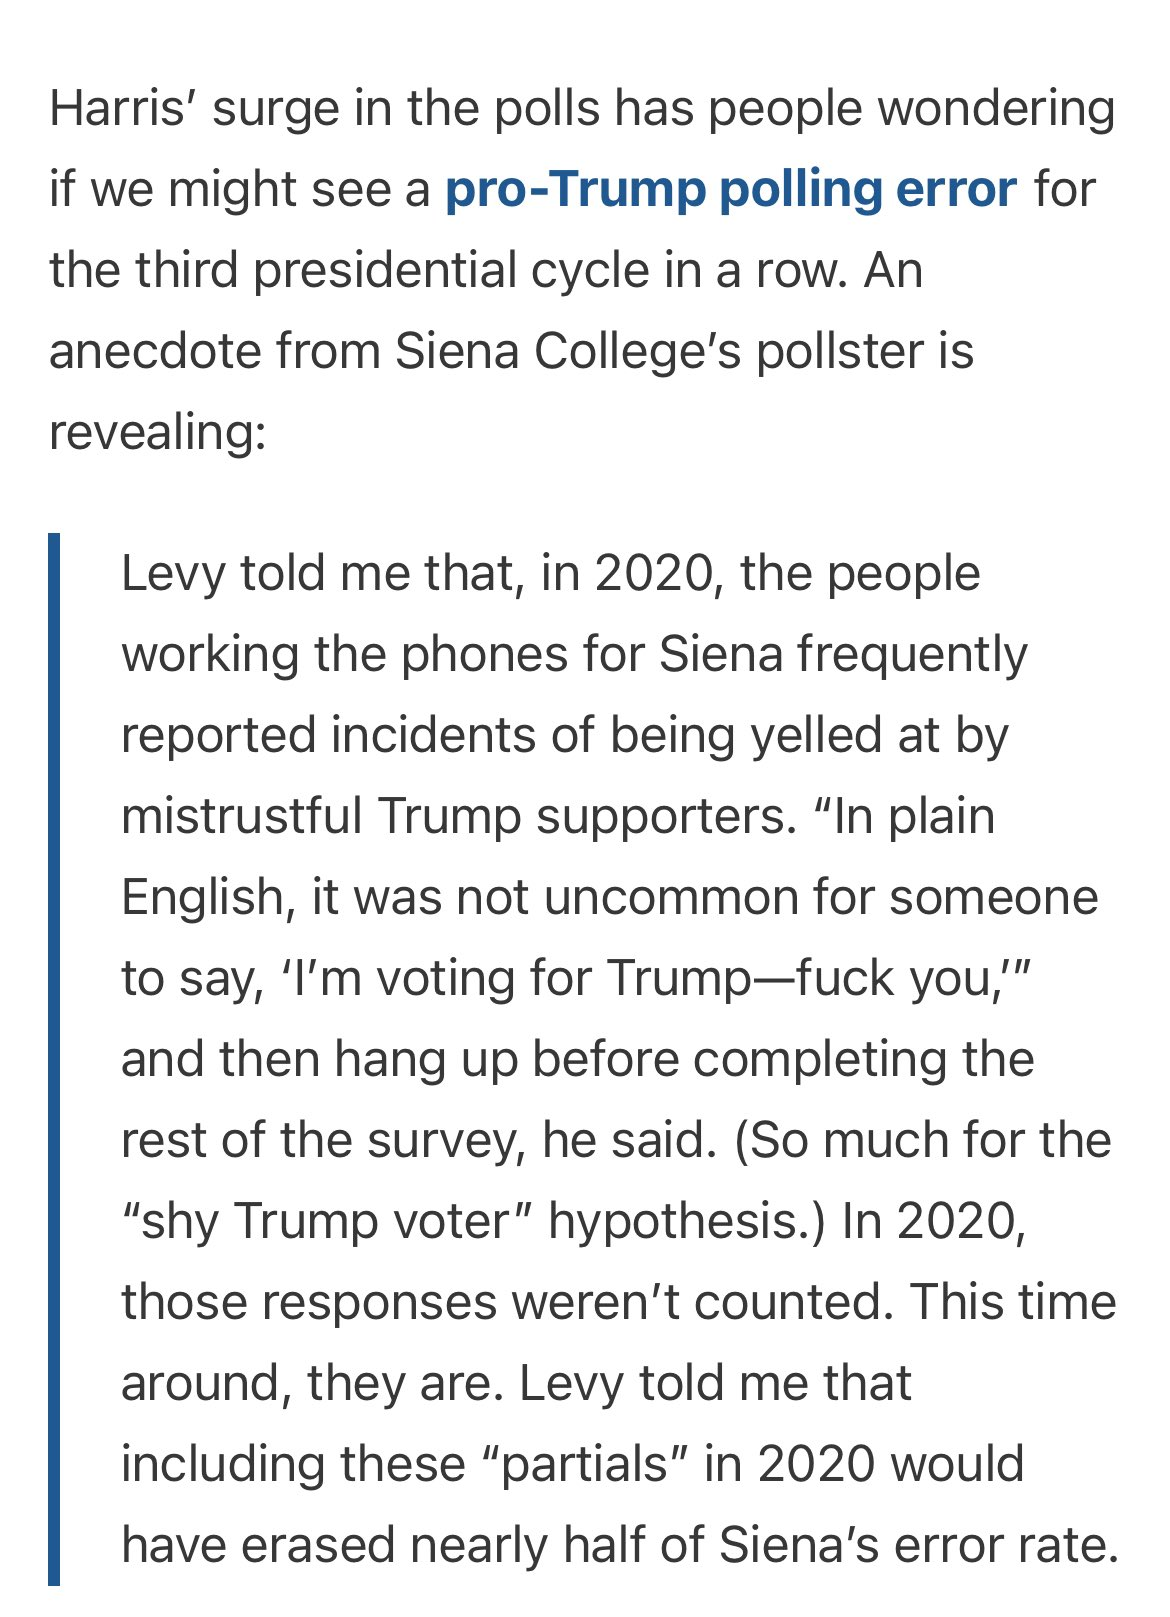
\includegraphics[width = .277\textwidth]{siena_polls.jpeg}}
    \fbox{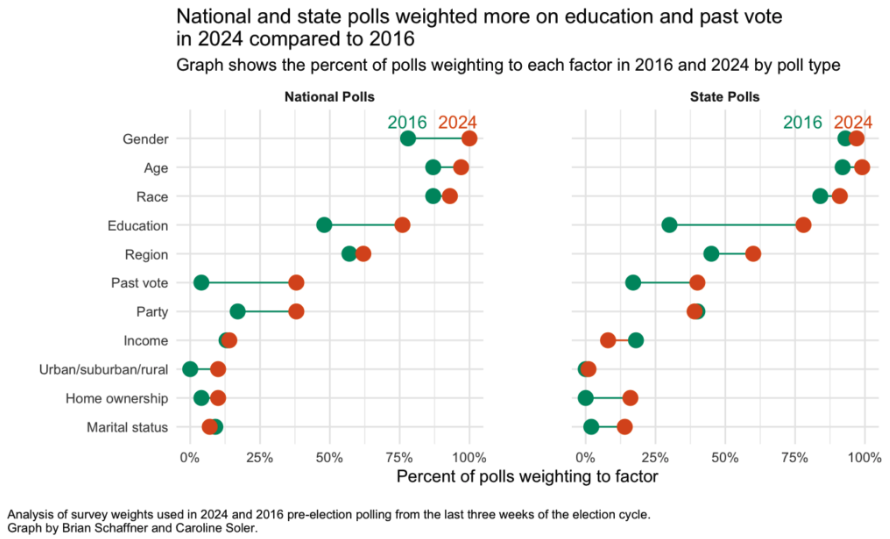
\includegraphics[width = .633\textwidth]{poll_weighting_factors.png}}
}

\only<4> {
    \centering
    ~\\
    \fbox{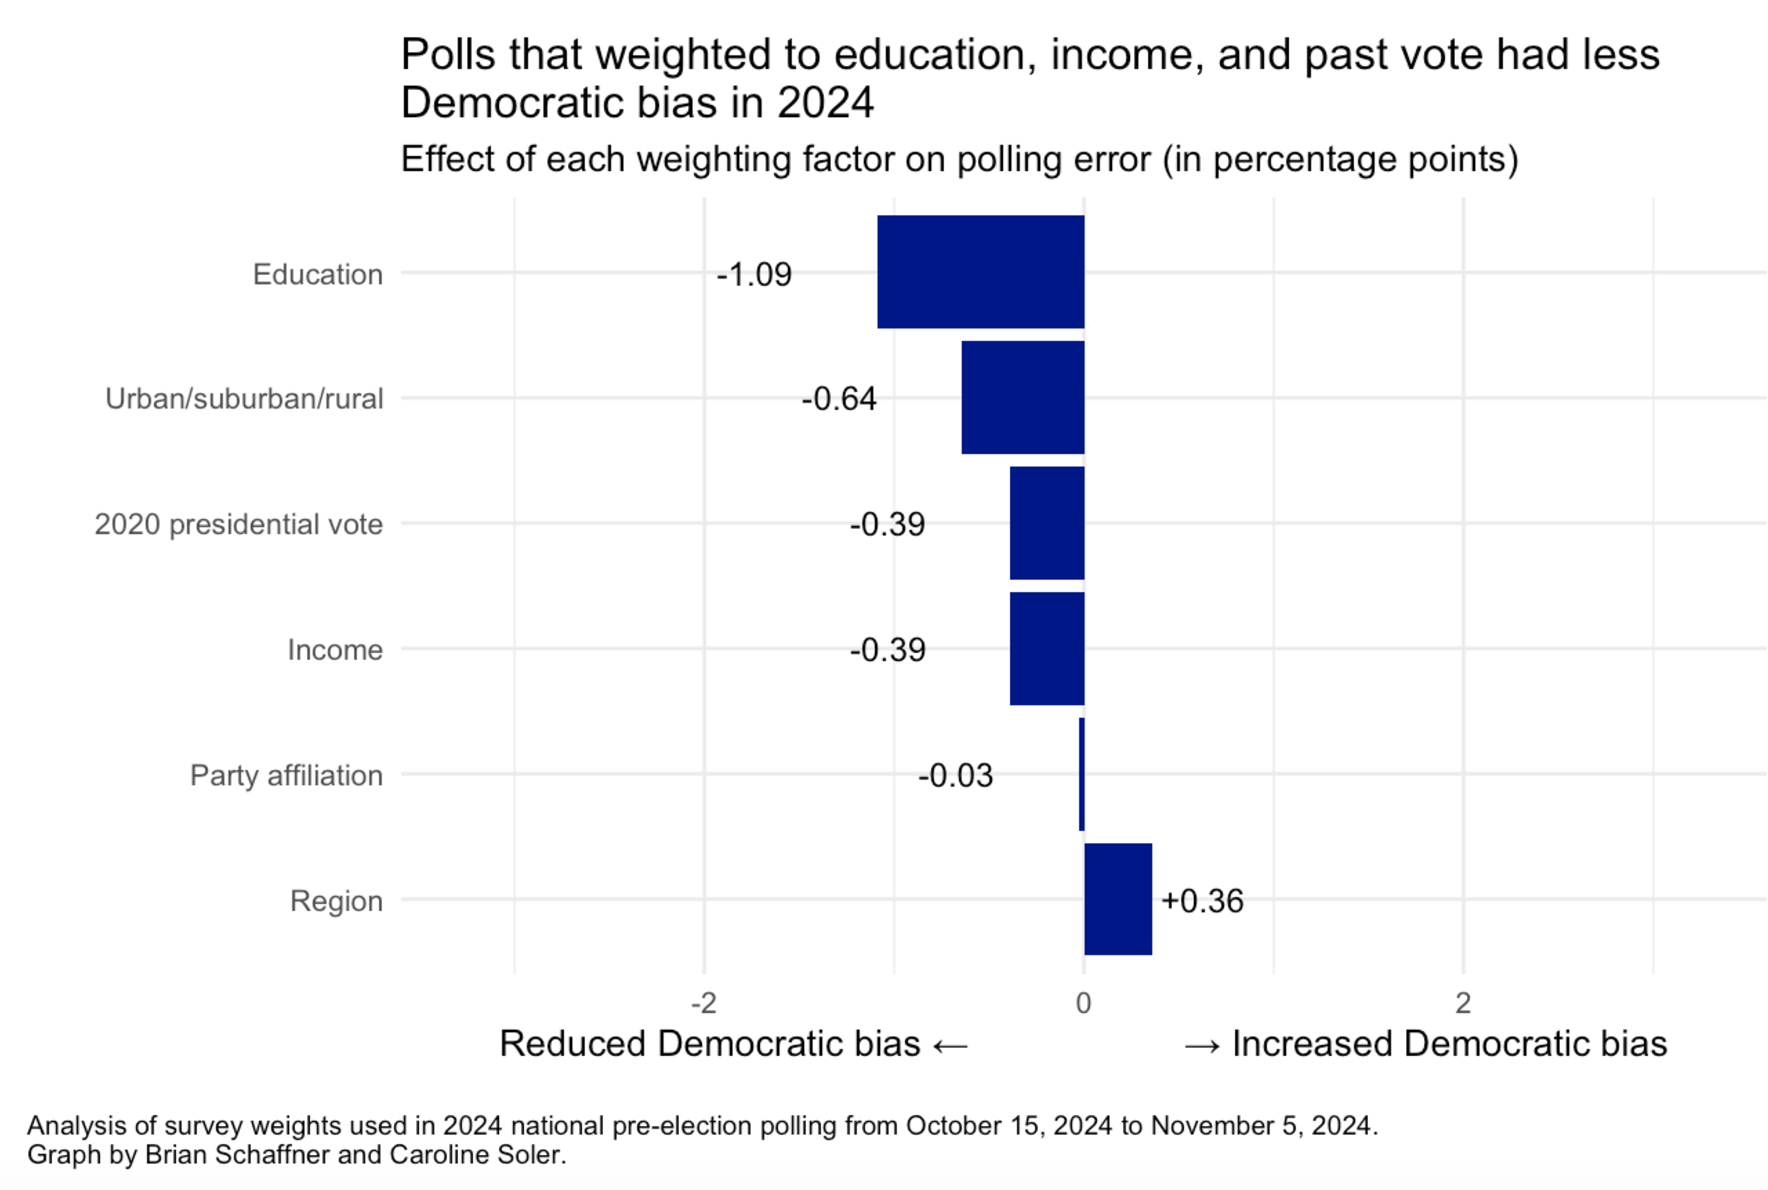
\includegraphics[width = .545\textwidth]{weighting_2024.png}}
    \fbox{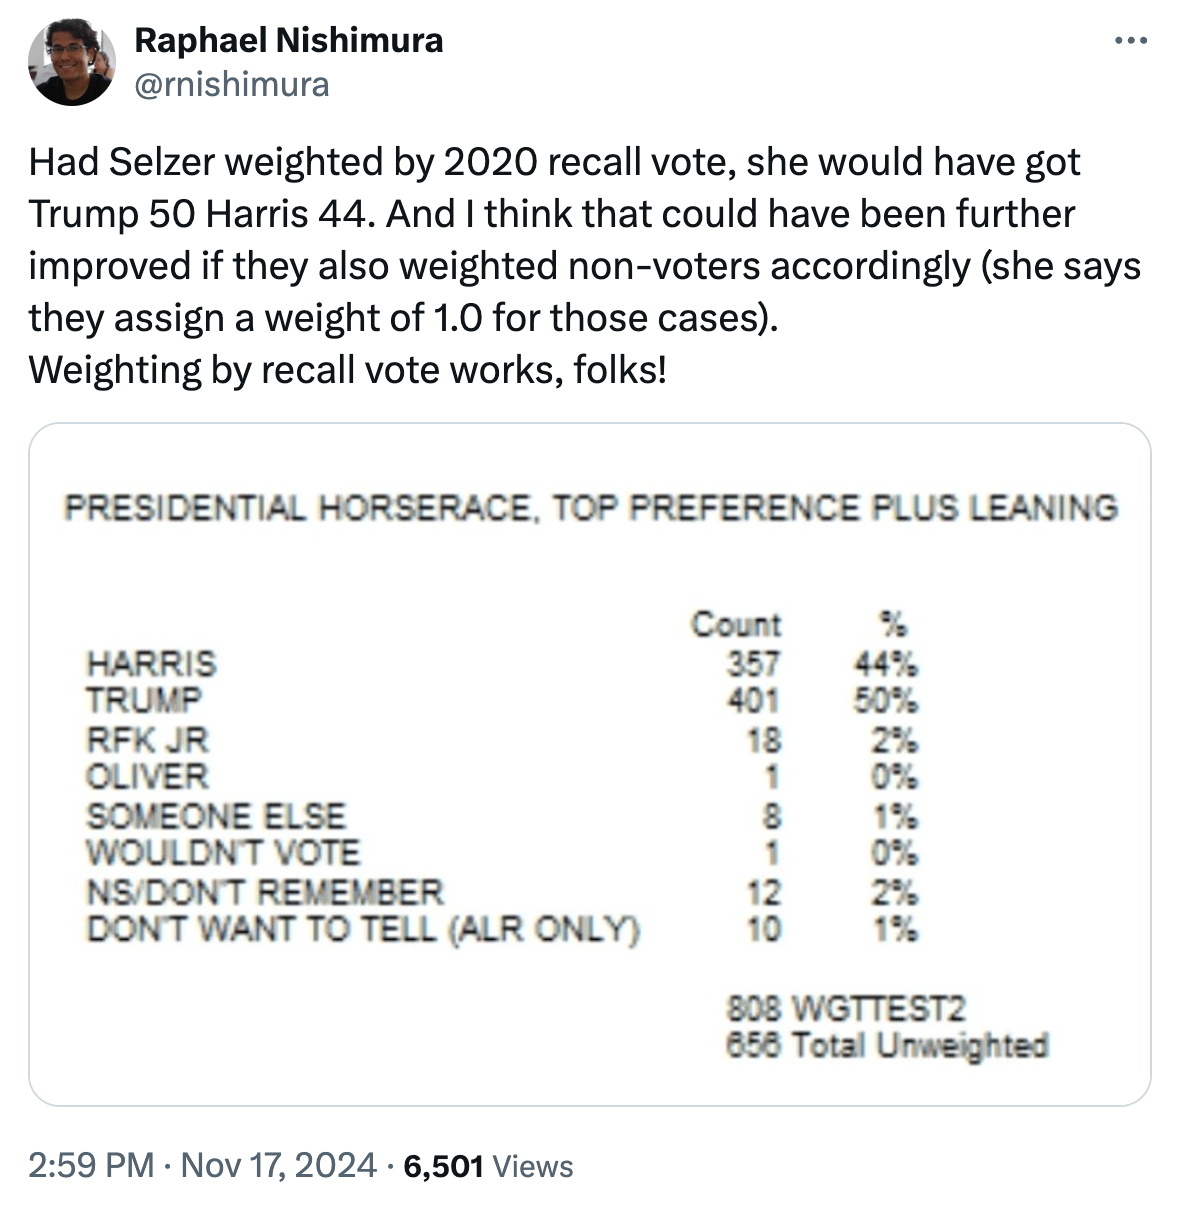
\includegraphics[width = .3575\textwidth]{selzer.png}}
}

\only<5>{
    \begin{itemize}
        \item Pollsters used new techniques to address partisan non-response, like weighting on \textbf{recalled vote}
        \item Recalled vote weighting assumes that the electorate looks the same from year-to-year
    \end{itemize}
}

\only<5>{
    \centering
    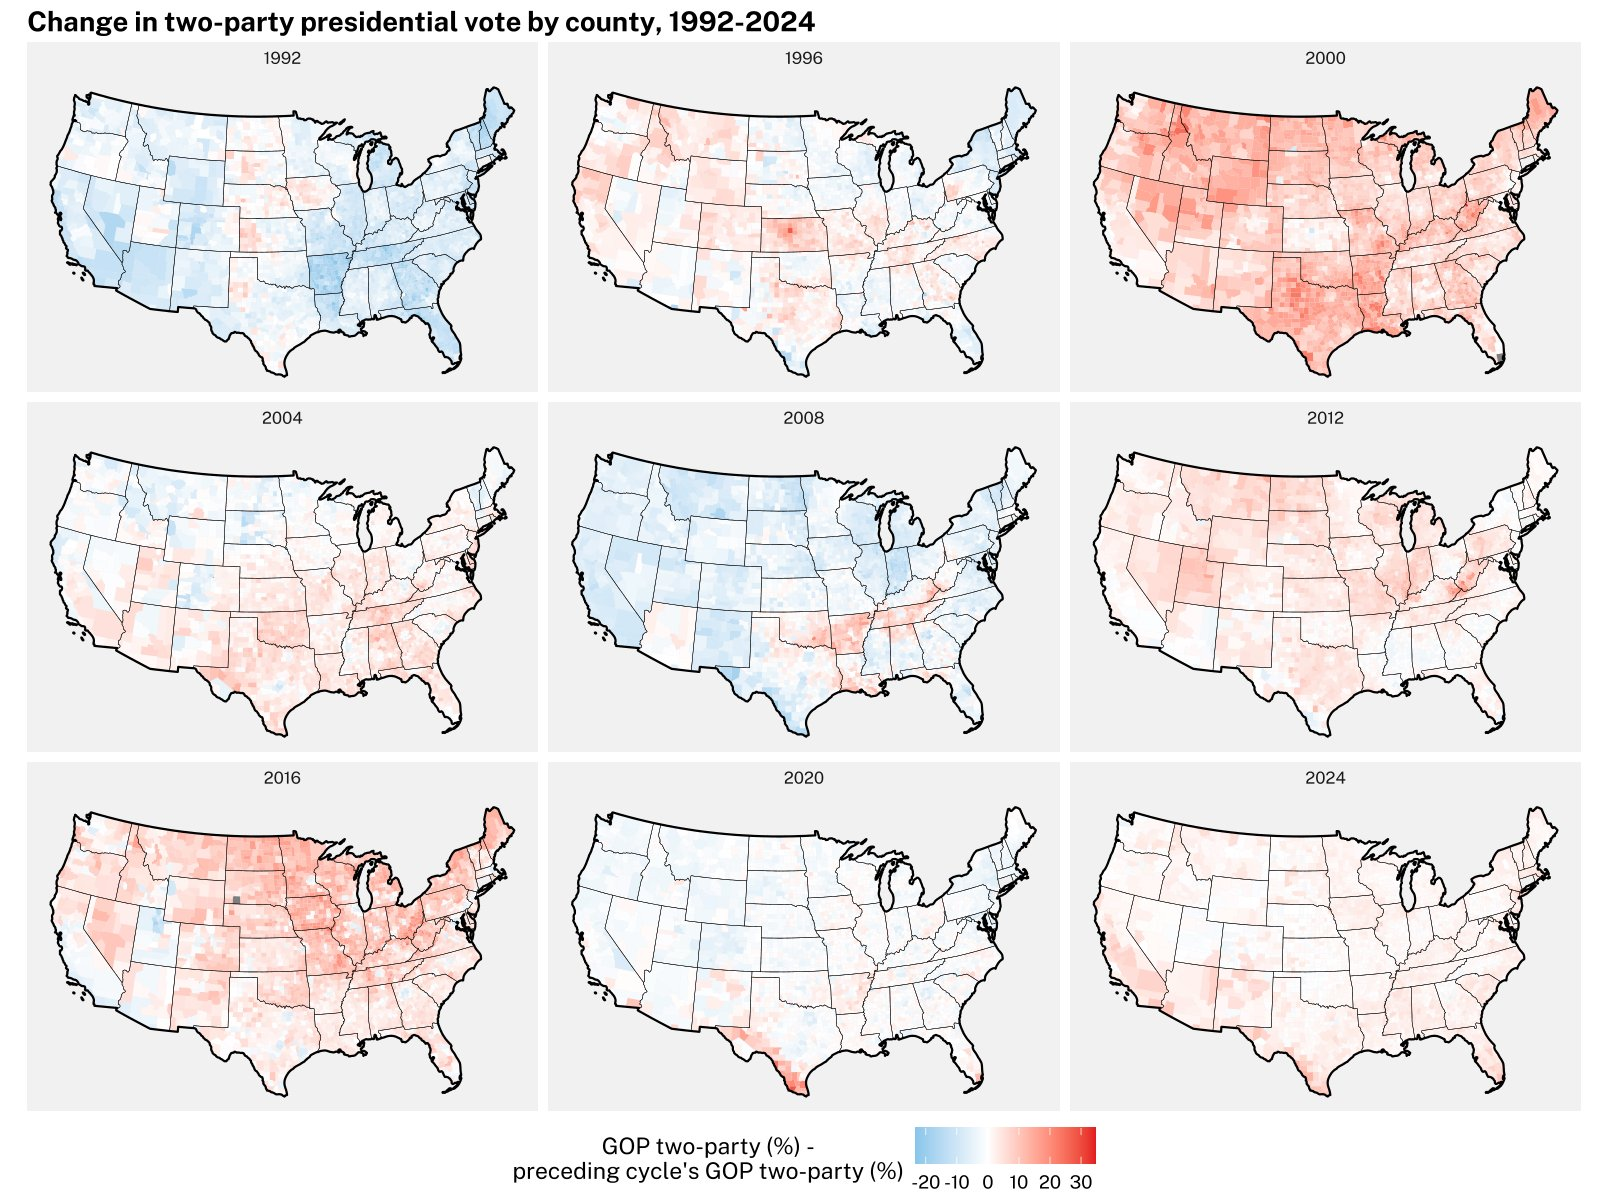
\includegraphics[height = .6\textheight]{vote_shift.jpeg}
}

\only<6->{
    \begin{itemize}
        \item Pollsters used new techniques to address partisan non-response, like weighting on \textbf{recalled vote}
        \item Recalled vote weighting assumes that the electorate looks the same from year-to-year
        \item This is especially the case as pollsters begin using ``likely voter'' models
    \end{itemize}
}

\only<6>{
    \centering
    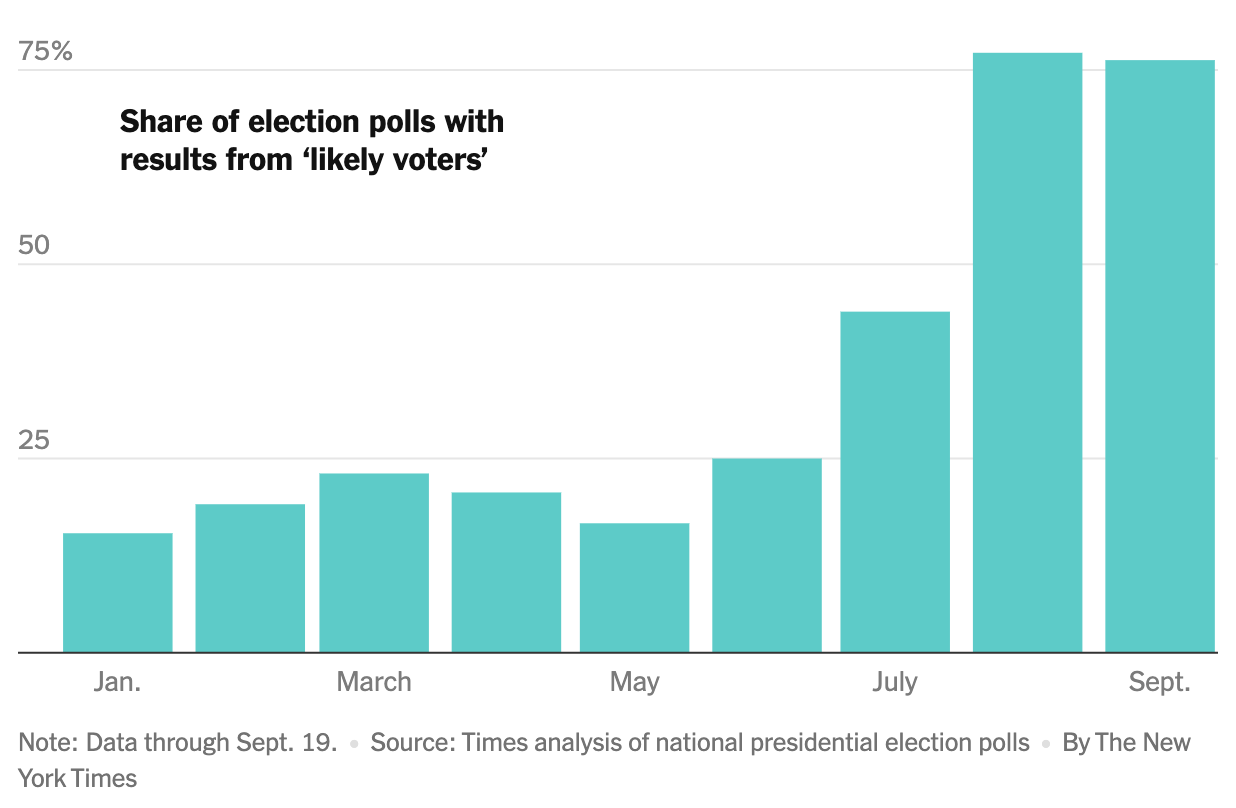
\includegraphics[height = .55\textheight]{lv_vs_rv.png}
}

\only<7>{
    \centering
    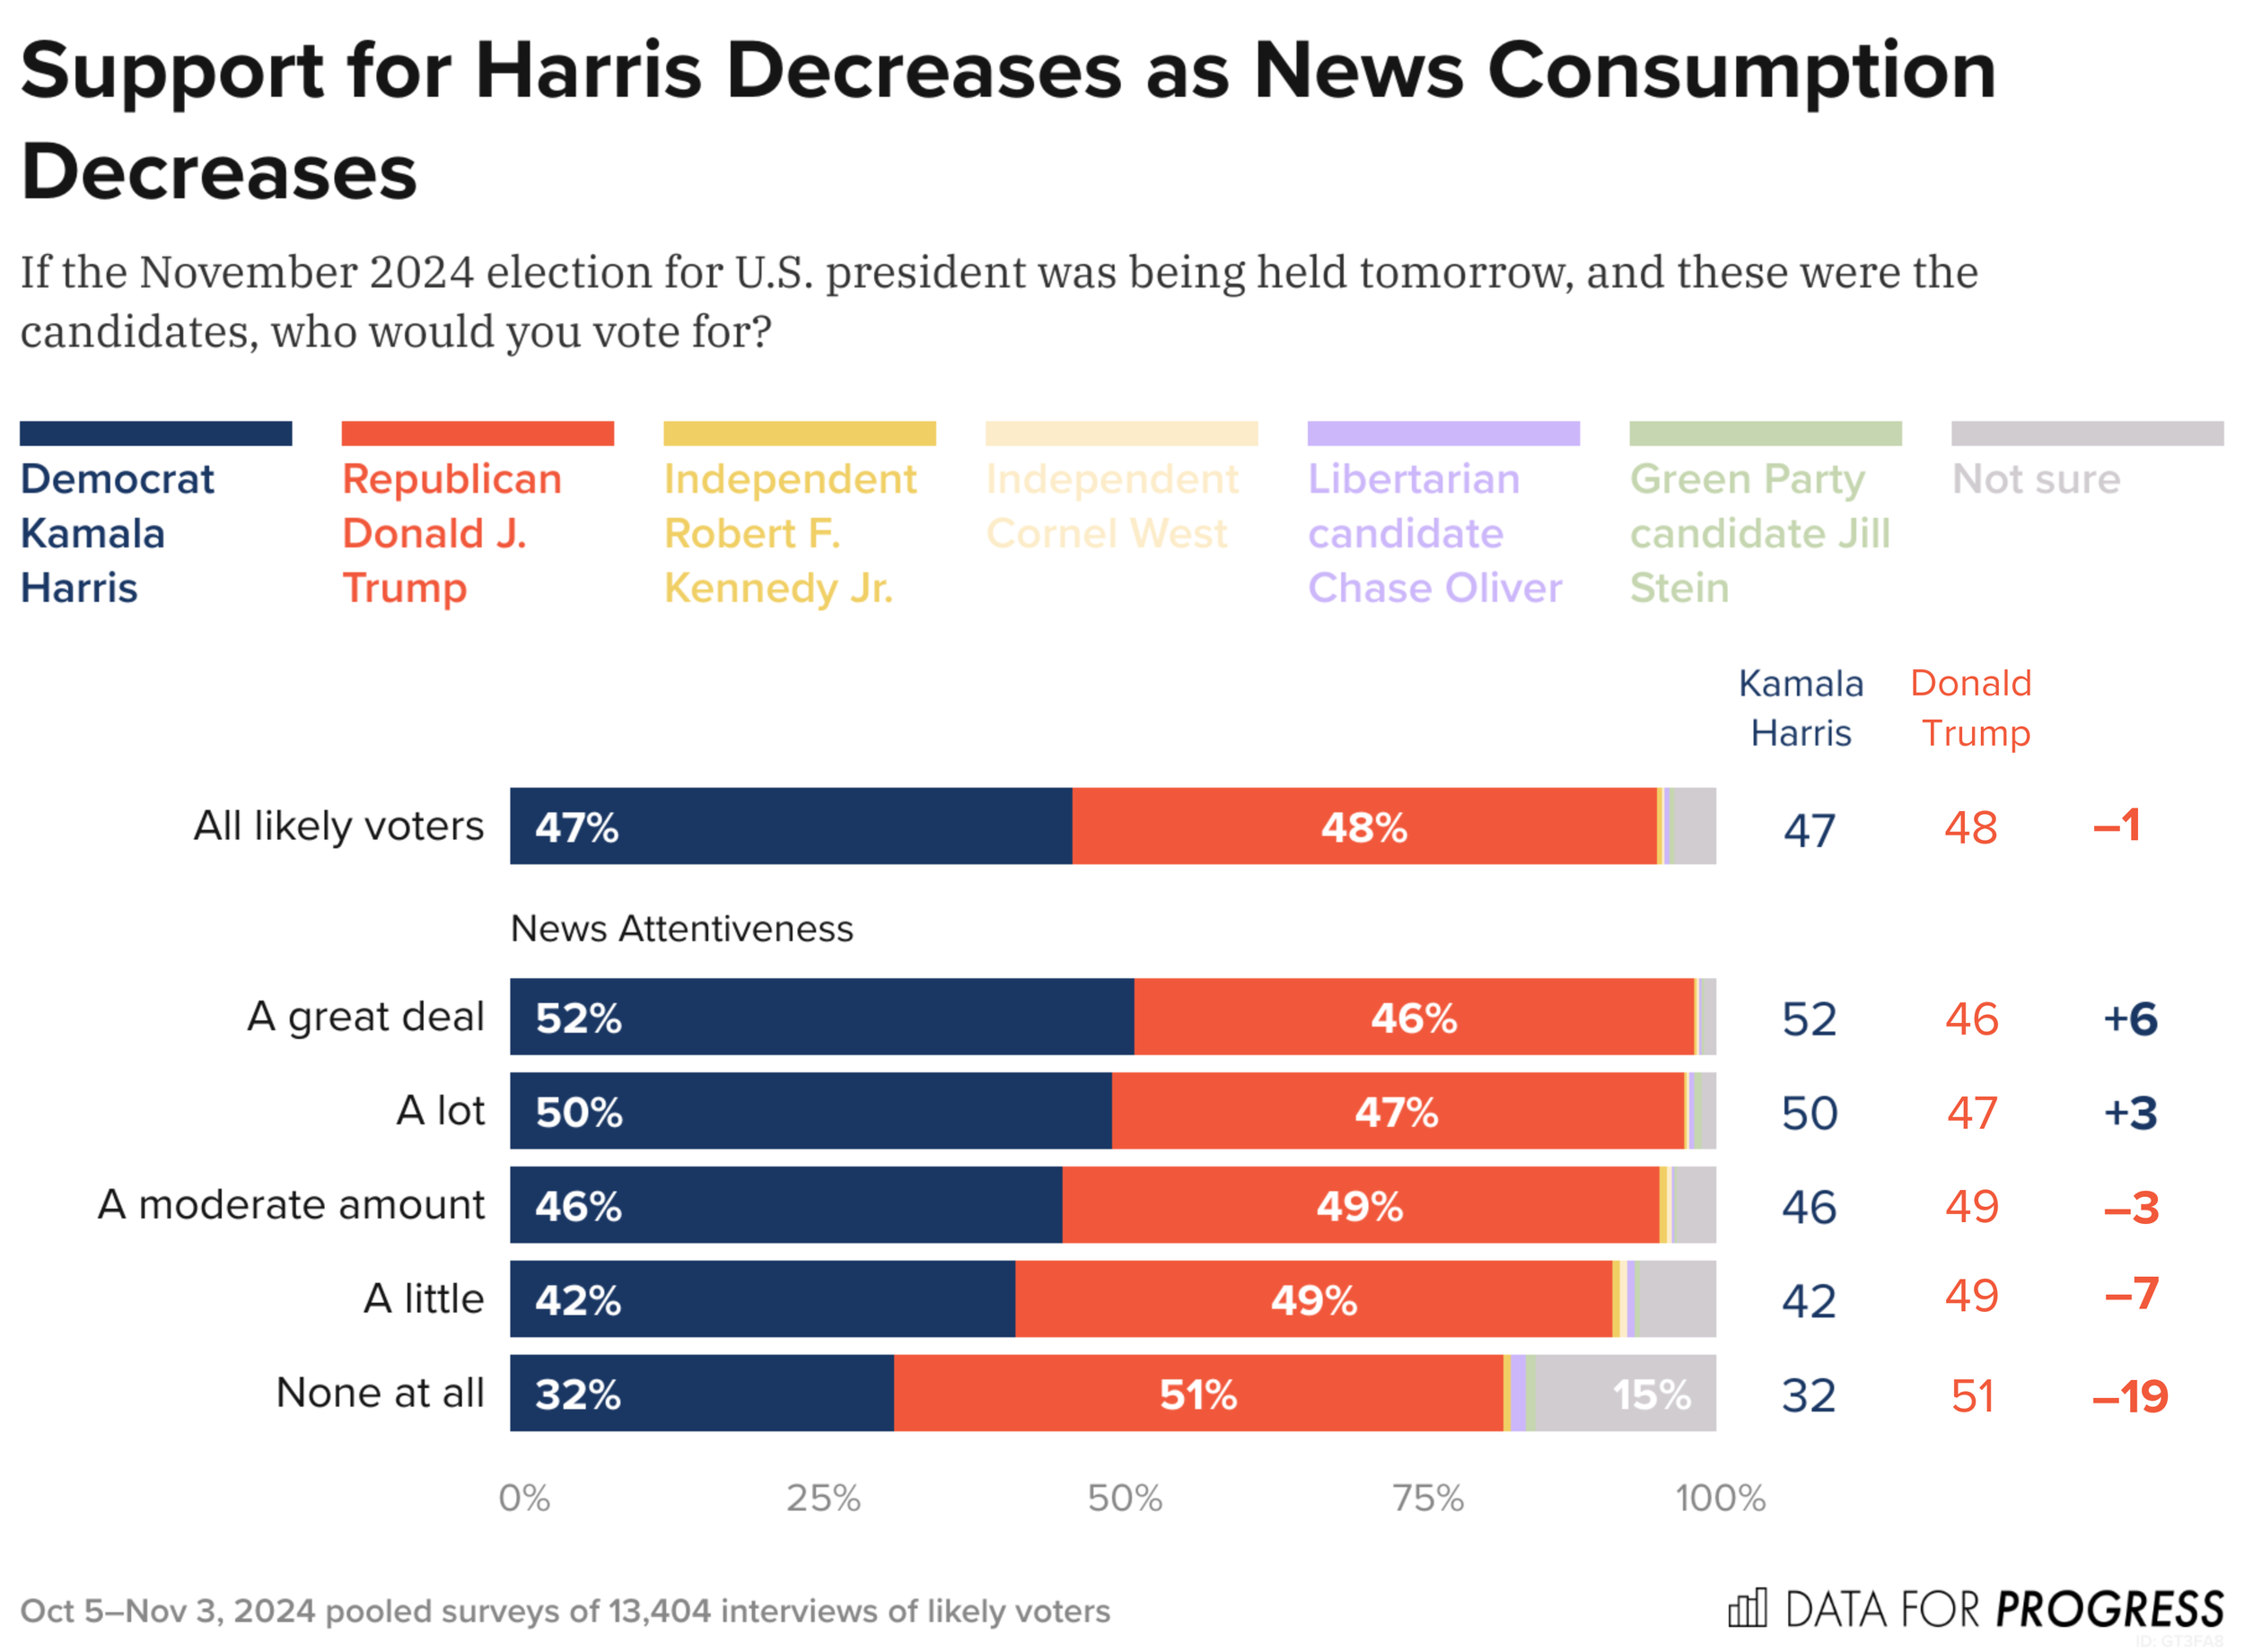
\includegraphics[height = .55\textheight]{news_consumption.png}
}

\only<8>{
    \centering
    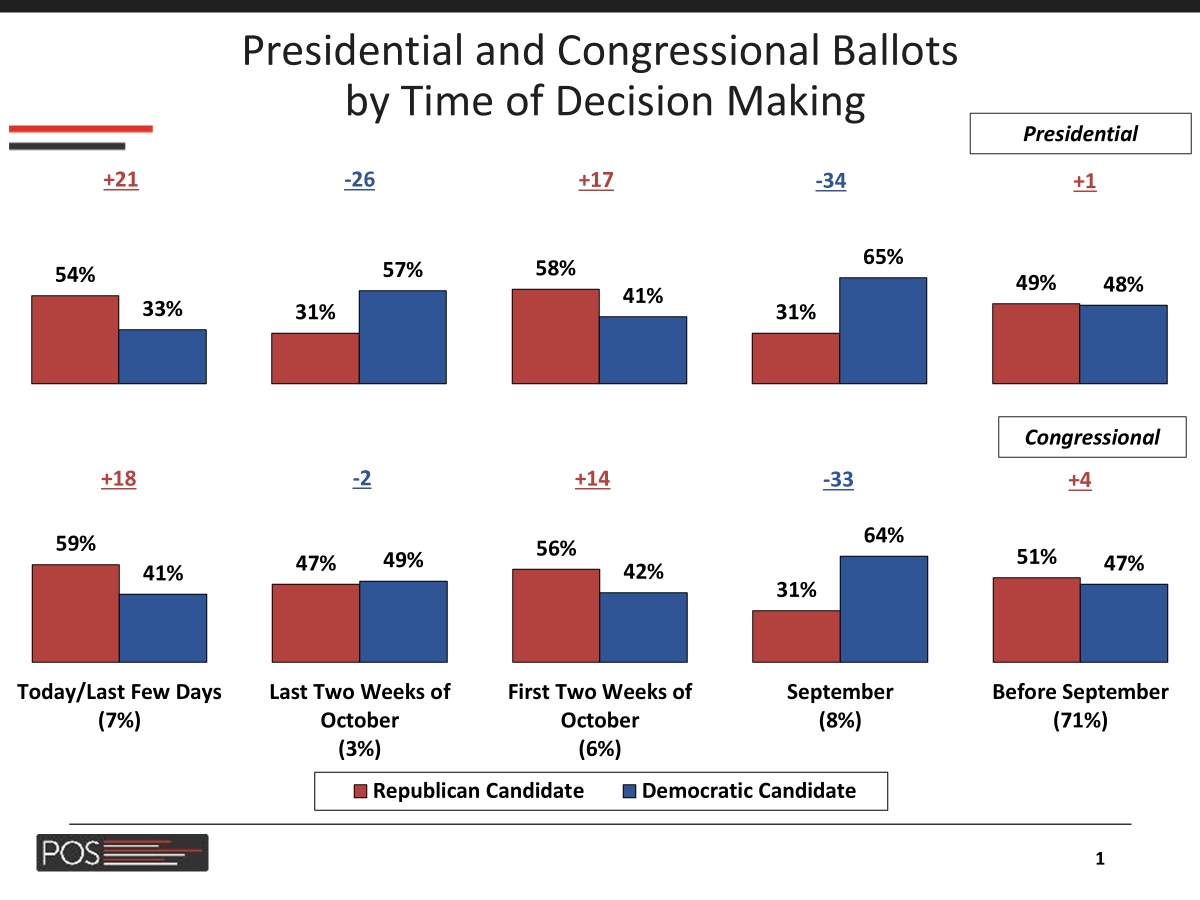
\includegraphics[height = .55\textheight]{late_deciders.png}
}
}

%%%%%%%%%%%%%%%%%%%%%%%%%%%%%%%%%%%%%%%%%%%%%%%%%%%%%%%%%%%%%%%%%%
\frame{\frametitle{Polling Challenges}
\begin{table}[h]
    \centering
    \begin{tabular}{|p{0.3\linewidth} | p{0.6\linewidth}|}
        \hline
        2016 Presidential & Polls wrong due to \textbf{missing at \mbox{random} (MAR)} non-response bias by education \\
        \hline
        2020 Presidential  & Polls wrong due to \textbf{missing not at random (MNAR)} non-response bias \\
        \hline
        2022 Midterm  & The rise of partisan polling and \mbox{\textbf{herding}} \\
        \hline
        2024 Presidential & Pollsters try weighting on \textbf{recalled vote} \\
        \hline
    \end{tabular}
\end{table}
}

\end{document}
